\documentclass[11pt,a4paper]{article}
\usepackage[utf8]{inputenc}
\usepackage[T1]{fontenc}
\usepackage[brazil]{babel}
\usepackage[a4paper,margin=2.5cm]{geometry}
\usepackage{graphicx}
\usepackage{booktabs}
\usepackage{float}
\usepackage{caption}
\usepackage{hyperref}
\hypersetup{colorlinks=true,linkcolor=blue,citecolor=blue,urlcolor=blue}

\title{Caracterizando a atividade de \emph{code review} no GitHub}
\author{Luiz Paulo Gon\c{c}alves \and Arthur Curi \and H\'elio Ernesto \\
PUC Minas -- Laborat\'orio de Experimenta\c{c}\~ao de Software \\
Prof. Danilo de Quadros Maia Filho}
\date{\today}

\begin{document}
\maketitle

\begin{abstract}
Este trabalho caracteriza a atividade de \emph{code review} em reposit\'orios populares do GitHub,
sob a perspectiva de quem submete c\'odigo. Coletamos 12.979 \emph{Pull Requests} a partir de
192 reposit\'orios entre os 200 mais populares por estrelas, contemplando apenas PRs com
status MERGED ou CLOSED, pelo menos uma revis\~ao registrada e tempo de an\'alise superior a uma hora.
Analisamos oito quest\~oes de pesquisa em duas dimens\~oes: o \emph{feedback} final da revis\~ao
(MERGED vs.\ CLOSED) e o n\'umero de revis\~oes realizadas, considerando como vari\'aveis
independentes o tamanho do PR, o tempo de an\'alise, a riqueza da descri\c{c}\~ao e o volume de
intera\c{c}\~oes. Utilizamos o teste de correla\c{c}\~ao de Spearman, adequado a dados
n\~ao-normais e \`a presen\c{c}a de \emph{outliers}, e reportamos coeficiente $\rho$ e
$p$-valor para cada RQ.
\end{abstract}

\section{Introdu\c{c}\~ao}

Revis\~ao de c\'odigo (\emph{code review}) tornou-se pr\'atica central no desenvolvimento
moderno, especialmente em projetos \emph{open source} hospedados no GitHub. Por meio de
\emph{Pull Requests}, contribuidores submetem mudan\c{c}as que s\~ao discutidas, comentadas e
eventualmente aceitas (\emph{merged}) ou rejeitadas (\emph{closed}). Compreender quais
caracter\'isticas dos PRs influenciam a aceita\c{c}\~ao e a quantidade de revis\~oes recebidas
\'e fundamental para que submissores escrevam contribui\c{c}\~oes mais efetivas.

Neste trabalho buscamos responder a oito quest\~oes de pesquisa organizadas em duas dimens\~oes:
(A) o \emph{feedback} final da revis\~ao --- representado pelo status MERGED ou CLOSED --- e
(B) o n\'umero de revis\~oes (\emph{reviews}) registradas no PR. Em cada dimens\~ao consideramos
quatro vari\'aveis independentes: tamanho, tempo de an\'alise, descri\c{c}\~ao e intera\c{c}\~oes.

\paragraph{Hip\'oteses informais.}
Antes de coletar os dados, formulamos as seguintes expectativas para cada RQ:

\medskip
\textbf{RQ01}: PRs maiores tendem a introduzir mais riscos e demandam revisao mais detalhada, logo esperamos que PRs com maior numero de arquivos alterados (e mais linhas modificadas) tenham menor probabilidade de serem aceitos.\\
\textbf{RQ02}: Esperamos correlacao negativa: PRs que permanecem muito tempo em revisao costumam indicar discussoes prolongadas ou problemas que tendem a culminar em fechamento sem merge.\\
\textbf{RQ03}: Esperamos correlacao positiva: descricoes mais detalhadas fornecem contexto aos revisores e facilitam a aceitacao do PR.\\
\textbf{RQ04}: Esperamos efeito misto: por um lado mais participantes e comentarios indicam atencao ao PR; por outro, podem refletir controversia e questionamentos, podendo correlacionar-se negativamente com o merge.\\
\textbf{RQ05}: Esperamos correlacao positiva: PRs maiores tendem a passar por mais rodadas de revisao.\\
\textbf{RQ06}: Esperamos correlacao positiva: quanto mais tempo em revisao, maior a oportunidade de novas revisoes ocorrerem.\\
\textbf{RQ07}: Esperamos correlacao negativa (ou pequena): descricoes ricas reduziriam duvidas e, portanto, a necessidade de rodadas adicionais de revisao.\\
\textbf{RQ08}: Esperamos correlacao positiva: PRs com mais participantes e comentarios devem demandar mais revisoes.

\section{Metodologia}

\subsection*{Constru\c{c}\~ao do \emph{dataset}}

Os dados foram obtidos via API GraphQL do GitHub (\url{https://api.github.com/graphql}).
Inicialmente listamos os 200 reposit\'orios p\'ublicos com mais estrelas, mantendo apenas
aqueles com pelo menos 100 \emph{Pull Requests} no estado MERGED ou CLOSED. Para cada
reposit\'orio coletamos os \emph{Pull Requests} mais recentes at\'e o limite configur\'avel
\texttt{PR\_LIMIT\_PER\_REPO} (configurado como 200 nesta execu\c{c}\~ao), parametro que
explicitamente controla o tempo de execu\c{c}\~ao da coleta.

Aplicamos os seguintes filtros sobre cada PR:

\begin{itemize}
  \item status \texttt{MERGED} ou \texttt{CLOSED};
  \item pelo menos uma revis\~ao registrada (\texttt{reviews.totalCount} $\geq 1$);
  \item tempo de an\'alise superior a uma hora --- diferen\c{c}a entre \texttt{createdAt}
        e a \'ultima atividade (\texttt{mergedAt} ou \texttt{closedAt}). Esse crit\'erio
        elimina PRs revisados de forma autom\'atica por \emph{bots} ou CI.
\end{itemize}

A coleta \'e robusta: trata \emph{rate limit} prim\'ario (pausa at\'e \texttt{resetAt}
quando o or\c{c}amento de pontos est\'a baixo), \emph{secondary rate limit} (\emph{retry}
com \emph{backoff} exponencial), e mant\'em \emph{checkpoint} por reposit\'orio (arquivos
JSON em \texttt{data/checkpoints/}), permitindo retomar de onde parou em caso de interrup\c{c}\~ao.

Ap\'os o filtro, o \emph{dataset} final cont\'em 12.979 PRs distribu\'idos em 192
reposit\'orios, dos quais 9.845 foram aceitos (MERGED) e 3.134 rejeitados (CLOSED).

\subsection*{M\'etricas por PR}

\begin{itemize}
  \item \textbf{Tamanho}: n\'umero de arquivos alterados (\texttt{changedFiles}) e total
        de linhas adicionadas mais removidas (\texttt{additions + deletions}).
  \item \textbf{Tempo de an\'alise}: intervalo em horas entre \texttt{createdAt} e
        \texttt{mergedAt}/\texttt{closedAt}.
  \item \textbf{Descri\c{c}\~ao}: n\'umero de caracteres do corpo do PR (\texttt{bodyText}).
  \item \textbf{Intera\c{c}\~oes}: \texttt{participants.totalCount} e
        \texttt{comments.totalCount}.
  \item \textbf{N\'umero de revis\~oes}: \texttt{reviews.totalCount}.
\end{itemize}

\subsection*{An\'alise estat\'istica}

Para cada RQ sumarizamos pelos valores \emph{medianos} sobre todos os PRs do \emph{dataset}
(sem agregar por reposit\'orio). Adotamos o teste de \textbf{correla\c{c}\~ao de Spearman} pelos
seguintes motivos:
(i) as distribui\c{c}\~oes das m\'etricas s\~ao fortemente assim\'etricas e apresentam
\emph{outliers} (tamanho e tempo costumam ter cauda longa);
(ii) n\~ao h\'a evid\^encia de normalidade --- requisito do teste de Pearson;
(iii) Spearman captura rela\c{c}\~oes monot\^onicas (e n\~ao apenas estritamente lineares),
o que \'e mais aderente \`a natureza dos dados de \emph{code review}.

Para as RQs da dimens\~ao A (status como vari\'avel dependente) codificamos o status como
bin\'ario (MERGED=1, CLOSED=0) e calculamos $\rho$ e $p$-valor entre a m\'etrica e o
status; tamb\'em reportamos as medianas das m\'etricas por grupo (MERGED vs.\ CLOSED).
Para as RQs da dimens\~ao B aplicamos Spearman diretamente entre a m\'etrica e
\texttt{reviews.totalCount}.

\section{Resultados}

A Tabela~\ref{tab:medianas} apresenta as medianas das m\'etricas, globais e por status.
A Tabela~\ref{tab:rqs} resume as correla\c{c}\~oes de Spearman para as oito RQs.

\begin{table}[H]
\centering
\caption{Medianas das m\'etricas globais e por status do PR.}
\label{tab:medianas}
\begin{tabular}{lrrr}
\toprule
M\'etrica & Geral & MERGED & CLOSED \\
\midrule
Arquivos alterados & 2,00 & 2,00 & 1,00 \\
Linhas alteradas (additions + deletions) & 37,00 & 38,00 & 32,00 \\
Tempo de analise (horas) & 32,02 & 24,50 & 102,03 \\
Tamanho da descricao (caracteres) & 659,00 & 640,00 & 696,50 \\
Numero de participantes & 2,00 & 2,00 & 2,00 \\
Numero de comentarios & 1,00 & 1,00 & 2,00 \\
Numero de revisoes & 1,00 & 2,00 & 1,00 \\
\bottomrule
\end{tabular}
\end{table}

\begin{table}[H]
\centering
\caption{Resumo das 8 RQs: correla\c{c}\~ao de Spearman entre cada m\'etrica e a vari\'avel dependente.}
\label{tab:rqs}
\begin{tabular}{llrrr}
\toprule
RQ & M\'etrica & $\rho$ & $p$-valor & $n$ \\
\midrule
RQ01 & arquivos alterados & $0{,}1089$ & $< 0{,}0001$ & 12.979 \\
RQ01 & linhas alteradas (additions + deletions) & $0{,}0299$ & $0{,}0006$ & 12.979 \\
RQ02 & tempo de analise (horas) & $-0{,}2272$ & $< 0{,}0001$ & 12.979 \\
RQ03 & tamanho da descricao (caracteres) & $-0{,}0167$ & $0{,}0576$ & 12.979 \\
RQ04 & numero de participantes & $-0{,}0205$ & $0{,}0194$ & 12.979 \\
RQ04 & numero de comentarios & $-0{,}0808$ & $< 0{,}0001$ & 12.979 \\
RQ05 & arquivos alterados & $0{,}2450$ & $< 0{,}0001$ & 12.979 \\
RQ05 & linhas alteradas (additions + deletions) & $0{,}2909$ & $< 0{,}0001$ & 12.979 \\
RQ06 & tempo de analise (horas) & $0{,}0777$ & $< 0{,}0001$ & 12.979 \\
RQ07 & tamanho da descricao (caracteres) & $0{,}1787$ & $< 0{,}0001$ & 12.979 \\
RQ08 & numero de participantes & $0{,}3504$ & $< 0{,}0001$ & 12.979 \\
RQ08 & numero de comentarios & $0{,}2899$ & $< 0{,}0001$ & 12.979 \\
\bottomrule
\end{tabular}
\end{table}

\subsection{Dimens\~ao A -- \emph{Feedback} final (MERGED vs.\ CLOSED)}

\subsection*{RQ01}
Para arquivos alterados, a mediana entre PRs aceitos (MERGED) foi 2,00 e entre rejeitados (CLOSED) foi 1,00. A correla\c{c}\~ao de Spearman com o status (MERGED=1, CLOSED=0) resultou em $\rho = 0{,}1089$ ($p\,< 0{,}0001$). Veja a Figura~\ref{fig:rq01_boxplot_changed_files}. Para linhas alteradas (additions + deletions), a mediana entre PRs aceitos (MERGED) foi 38,00 e entre rejeitados (CLOSED) foi 32,00. A correla\c{c}\~ao de Spearman com o status (MERGED=1, CLOSED=0) resultou em $\rho = 0{,}0299$ ($p\,= 0{,}0006$). Veja a Figura~\ref{fig:rq01_boxplot_lines_changed}.

\begin{figure}[H]
\centering
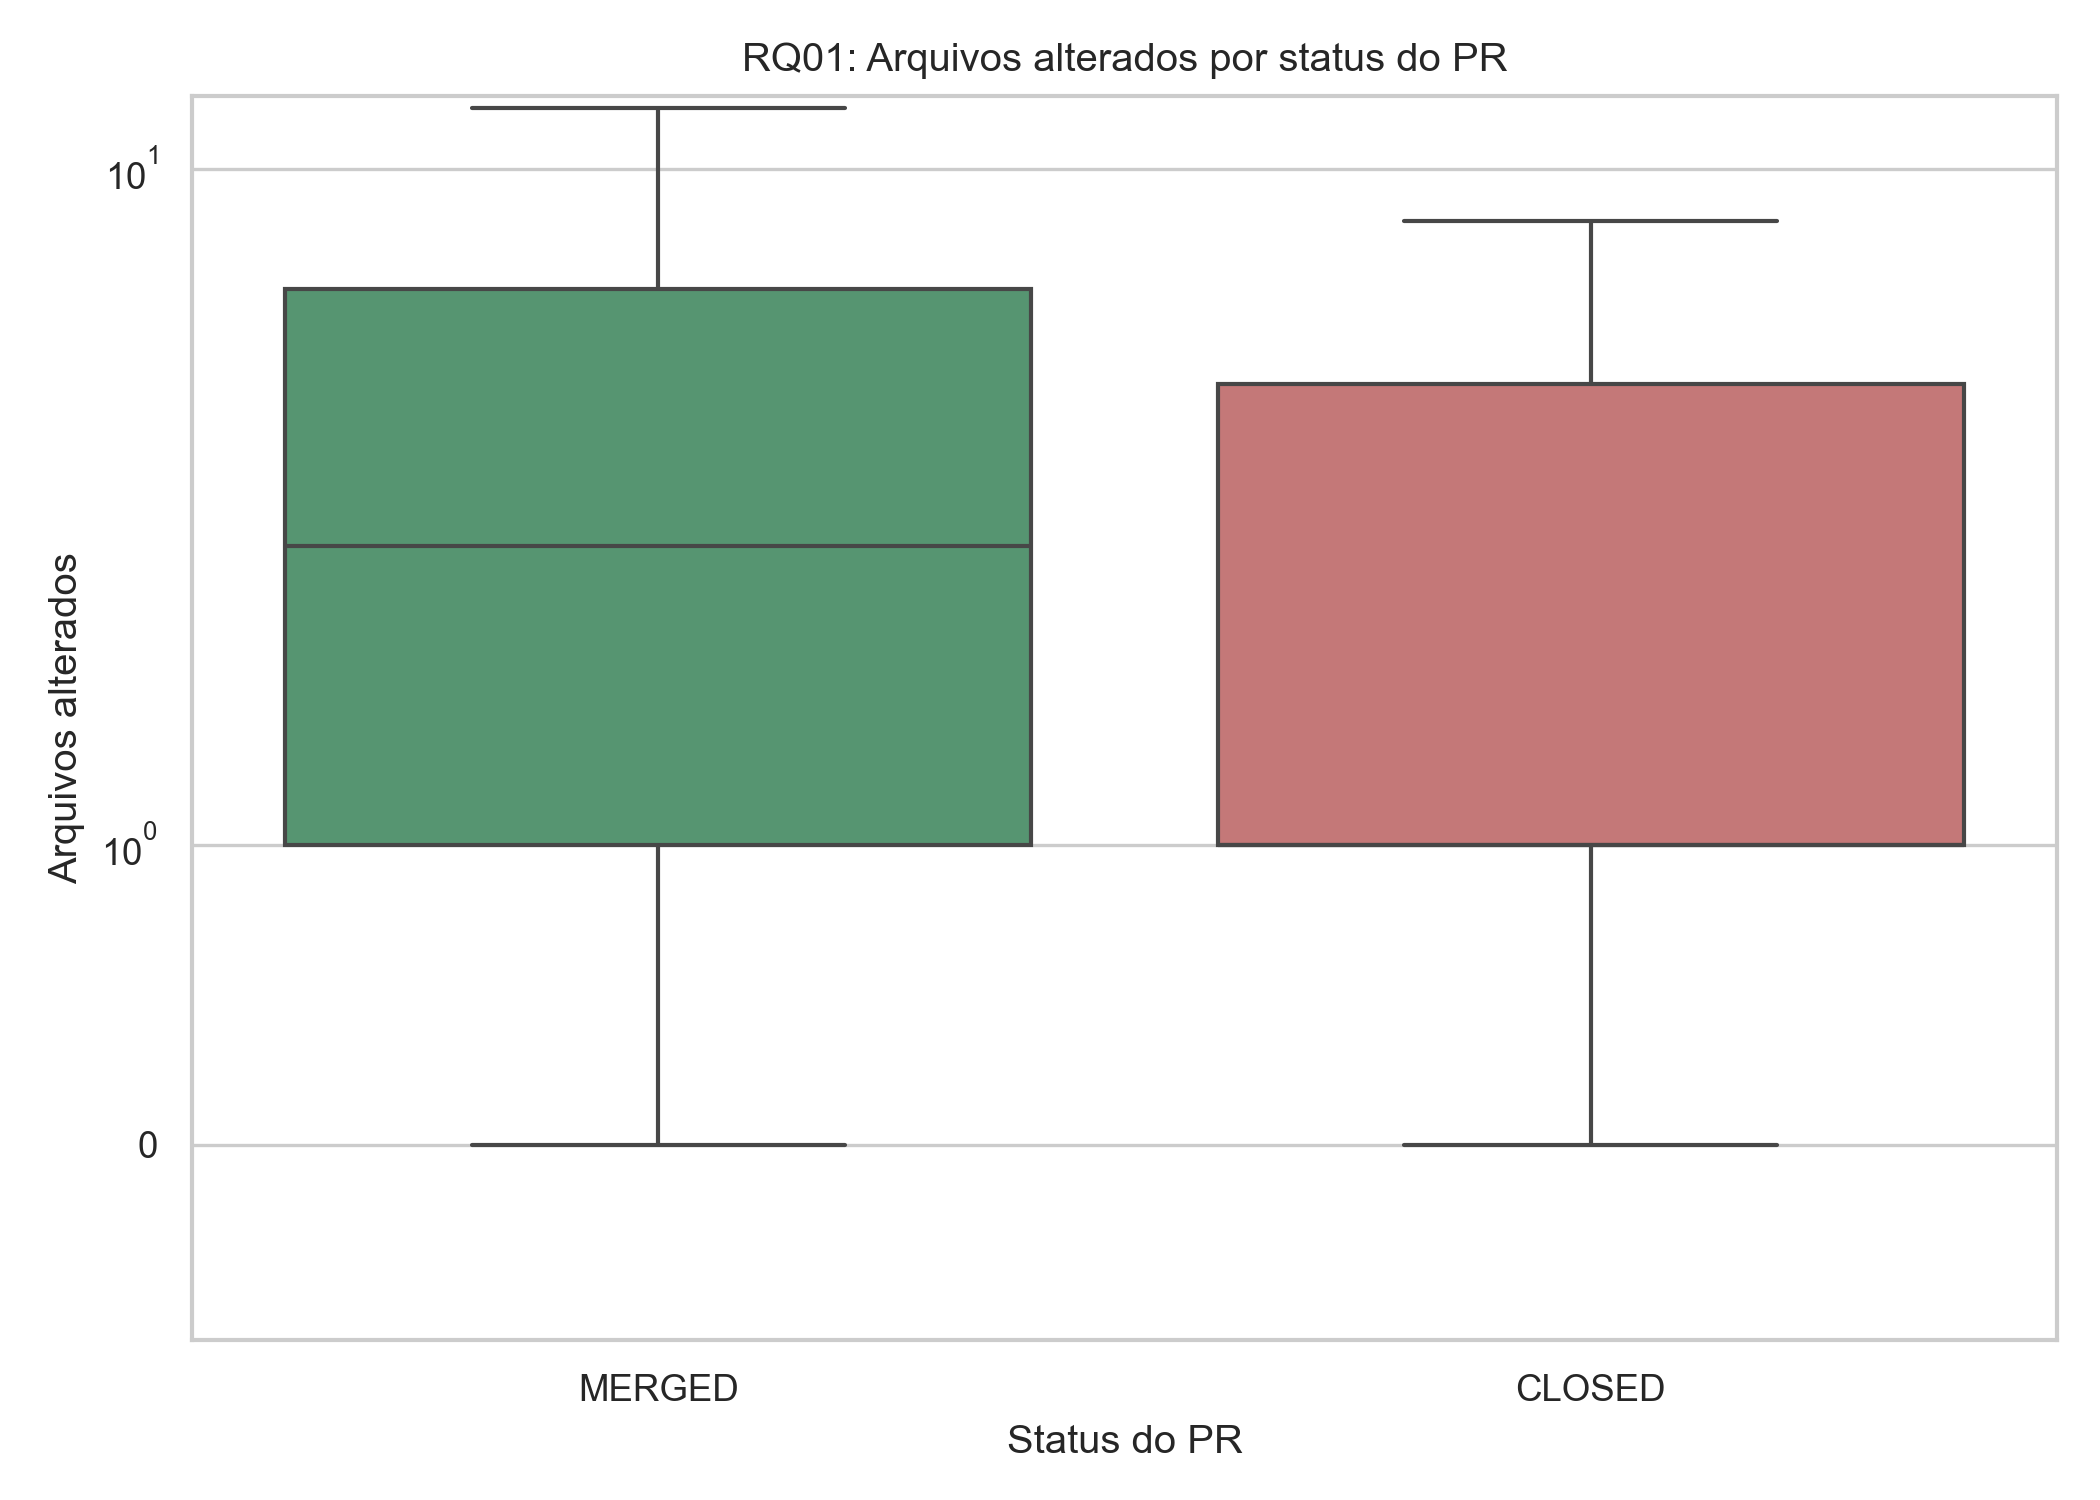
\includegraphics[width=0.78\textwidth]{../figures/rq01_boxplot_changed_files.png}
\caption{RQ01 - arquivos alterados}
\label{fig:rq01_boxplot_changed_files}
\end{figure}

\begin{figure}[H]
\centering
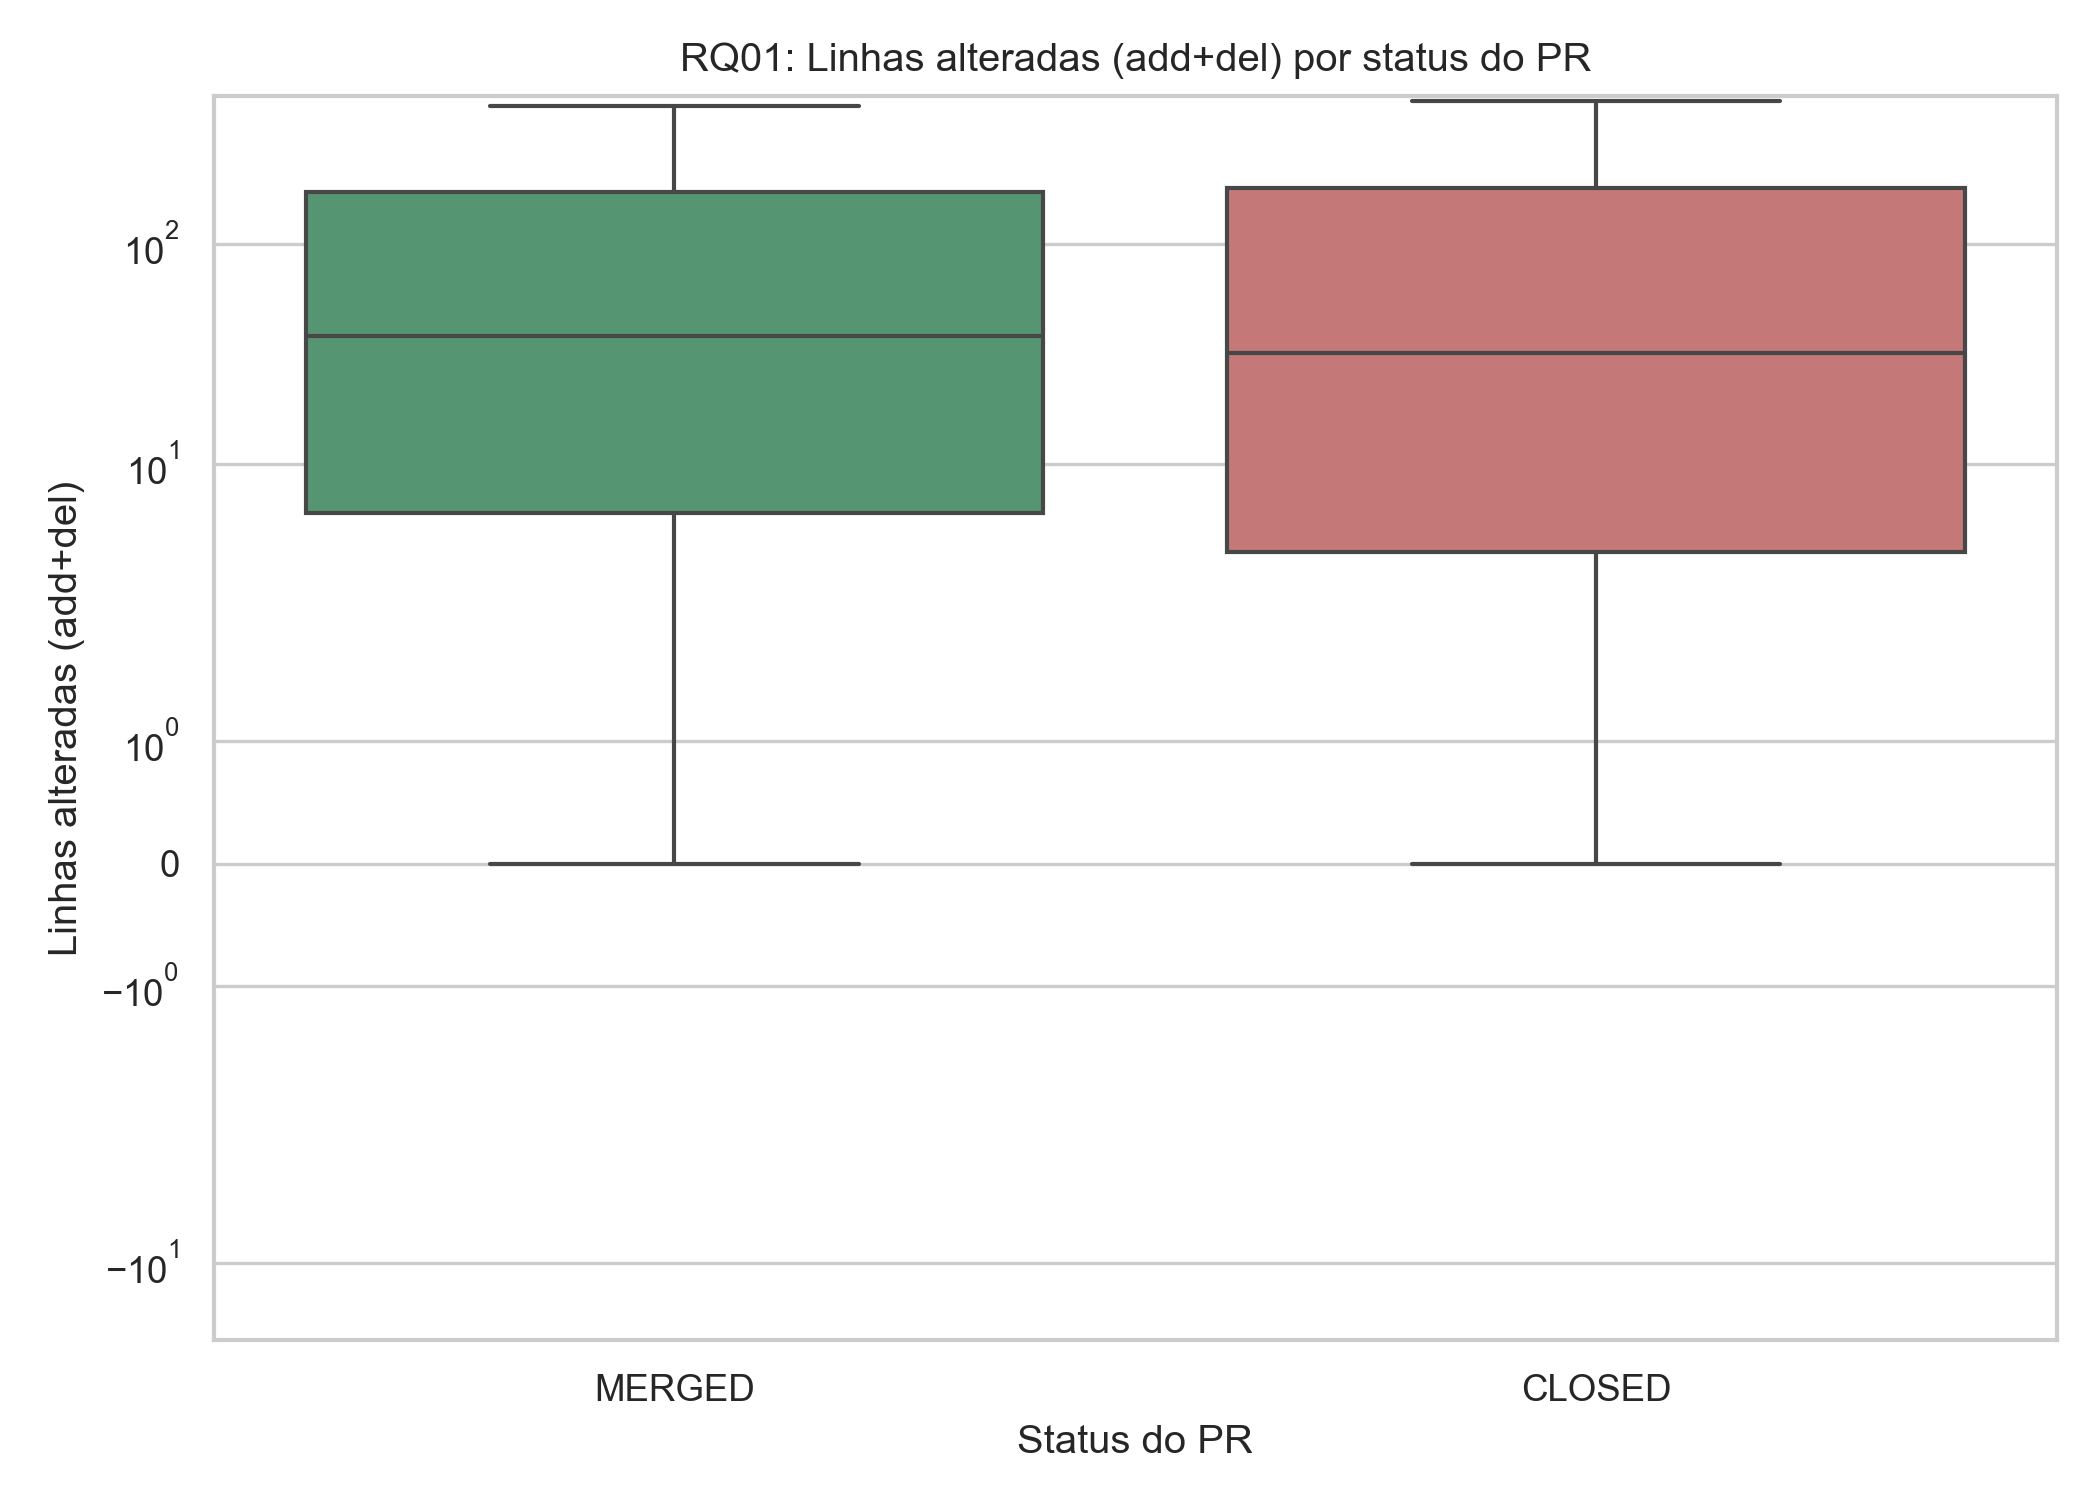
\includegraphics[width=0.78\textwidth]{../figures/rq01_boxplot_lines_changed.png}
\caption{RQ01 - linhas alteradas (additions + deletions)}
\label{fig:rq01_boxplot_lines_changed}
\end{figure}

\subsection*{RQ02}
Para tempo de analise (horas), a mediana entre PRs aceitos (MERGED) foi 24,50 e entre rejeitados (CLOSED) foi 102,03. A correla\c{c}\~ao de Spearman com o status (MERGED=1, CLOSED=0) resultou em $\rho = -0{,}2272$ ($p\,< 0{,}0001$). Veja a Figura~\ref{fig:rq02_boxplot_analysis_time_hours}.

\begin{figure}[H]
\centering
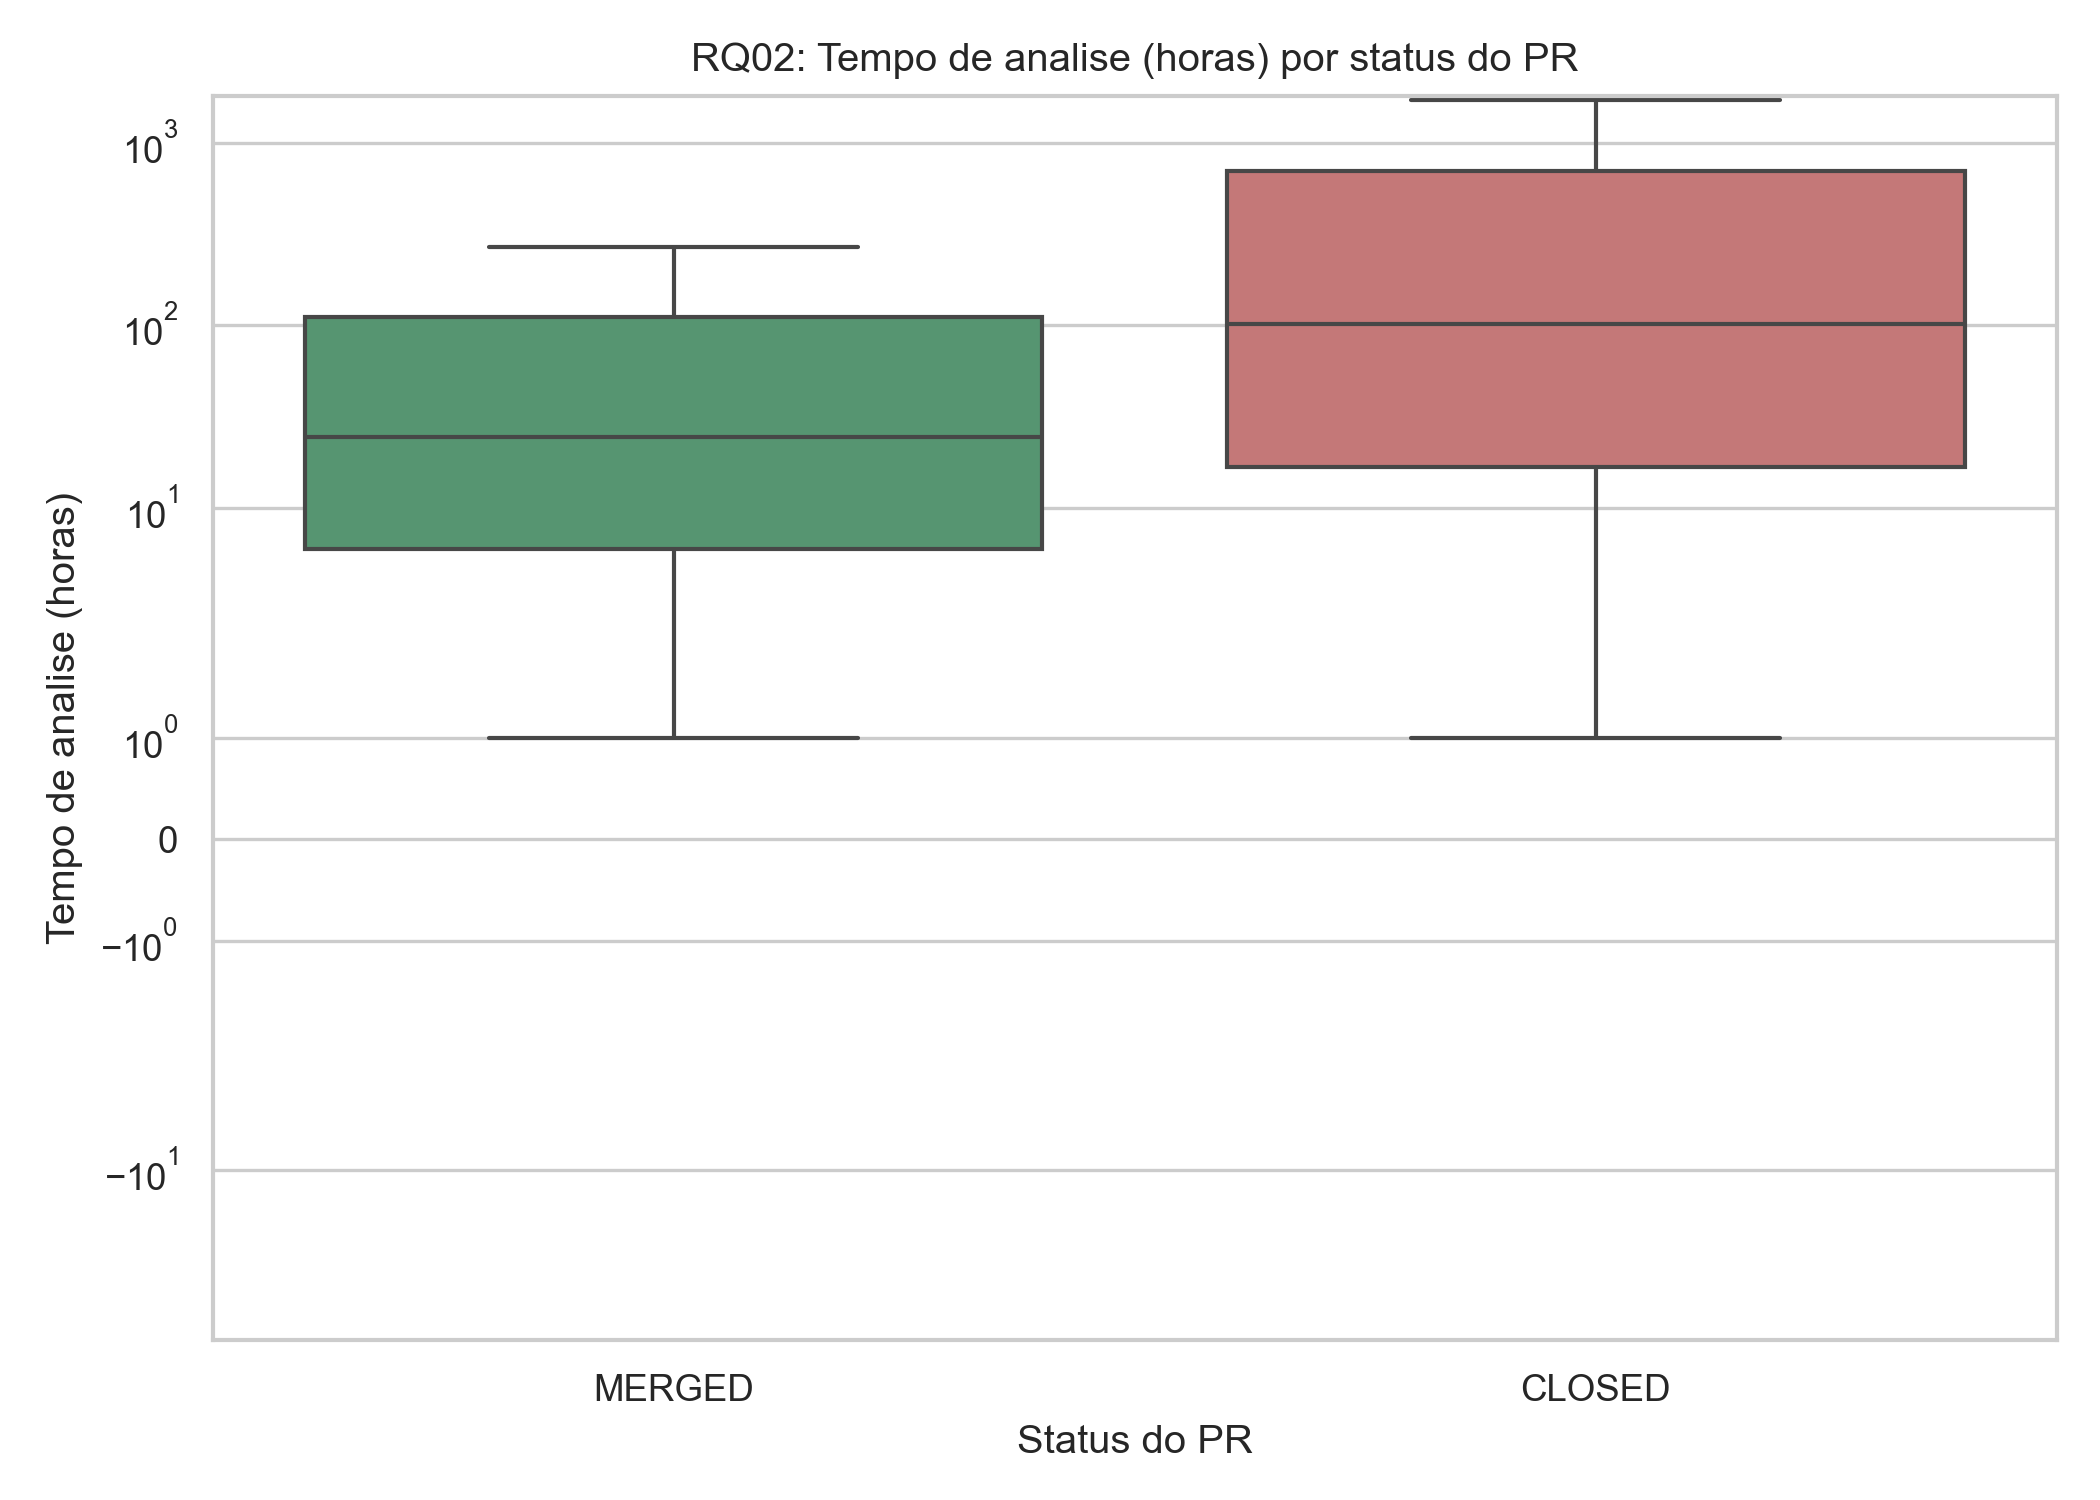
\includegraphics[width=0.78\textwidth]{../figures/rq02_boxplot_analysis_time_hours.png}
\caption{RQ02 - tempo de analise (horas)}
\label{fig:rq02_boxplot_analysis_time_hours}
\end{figure}

\subsection*{RQ03}
Para tamanho da descricao (caracteres), a mediana entre PRs aceitos (MERGED) foi 640,00 e entre rejeitados (CLOSED) foi 696,50. A correla\c{c}\~ao de Spearman com o status (MERGED=1, CLOSED=0) resultou em $\rho = -0{,}0167$ ($p\,= 0{,}0576$). Veja a Figura~\ref{fig:rq03_boxplot_body_length_chars}.

\begin{figure}[H]
\centering
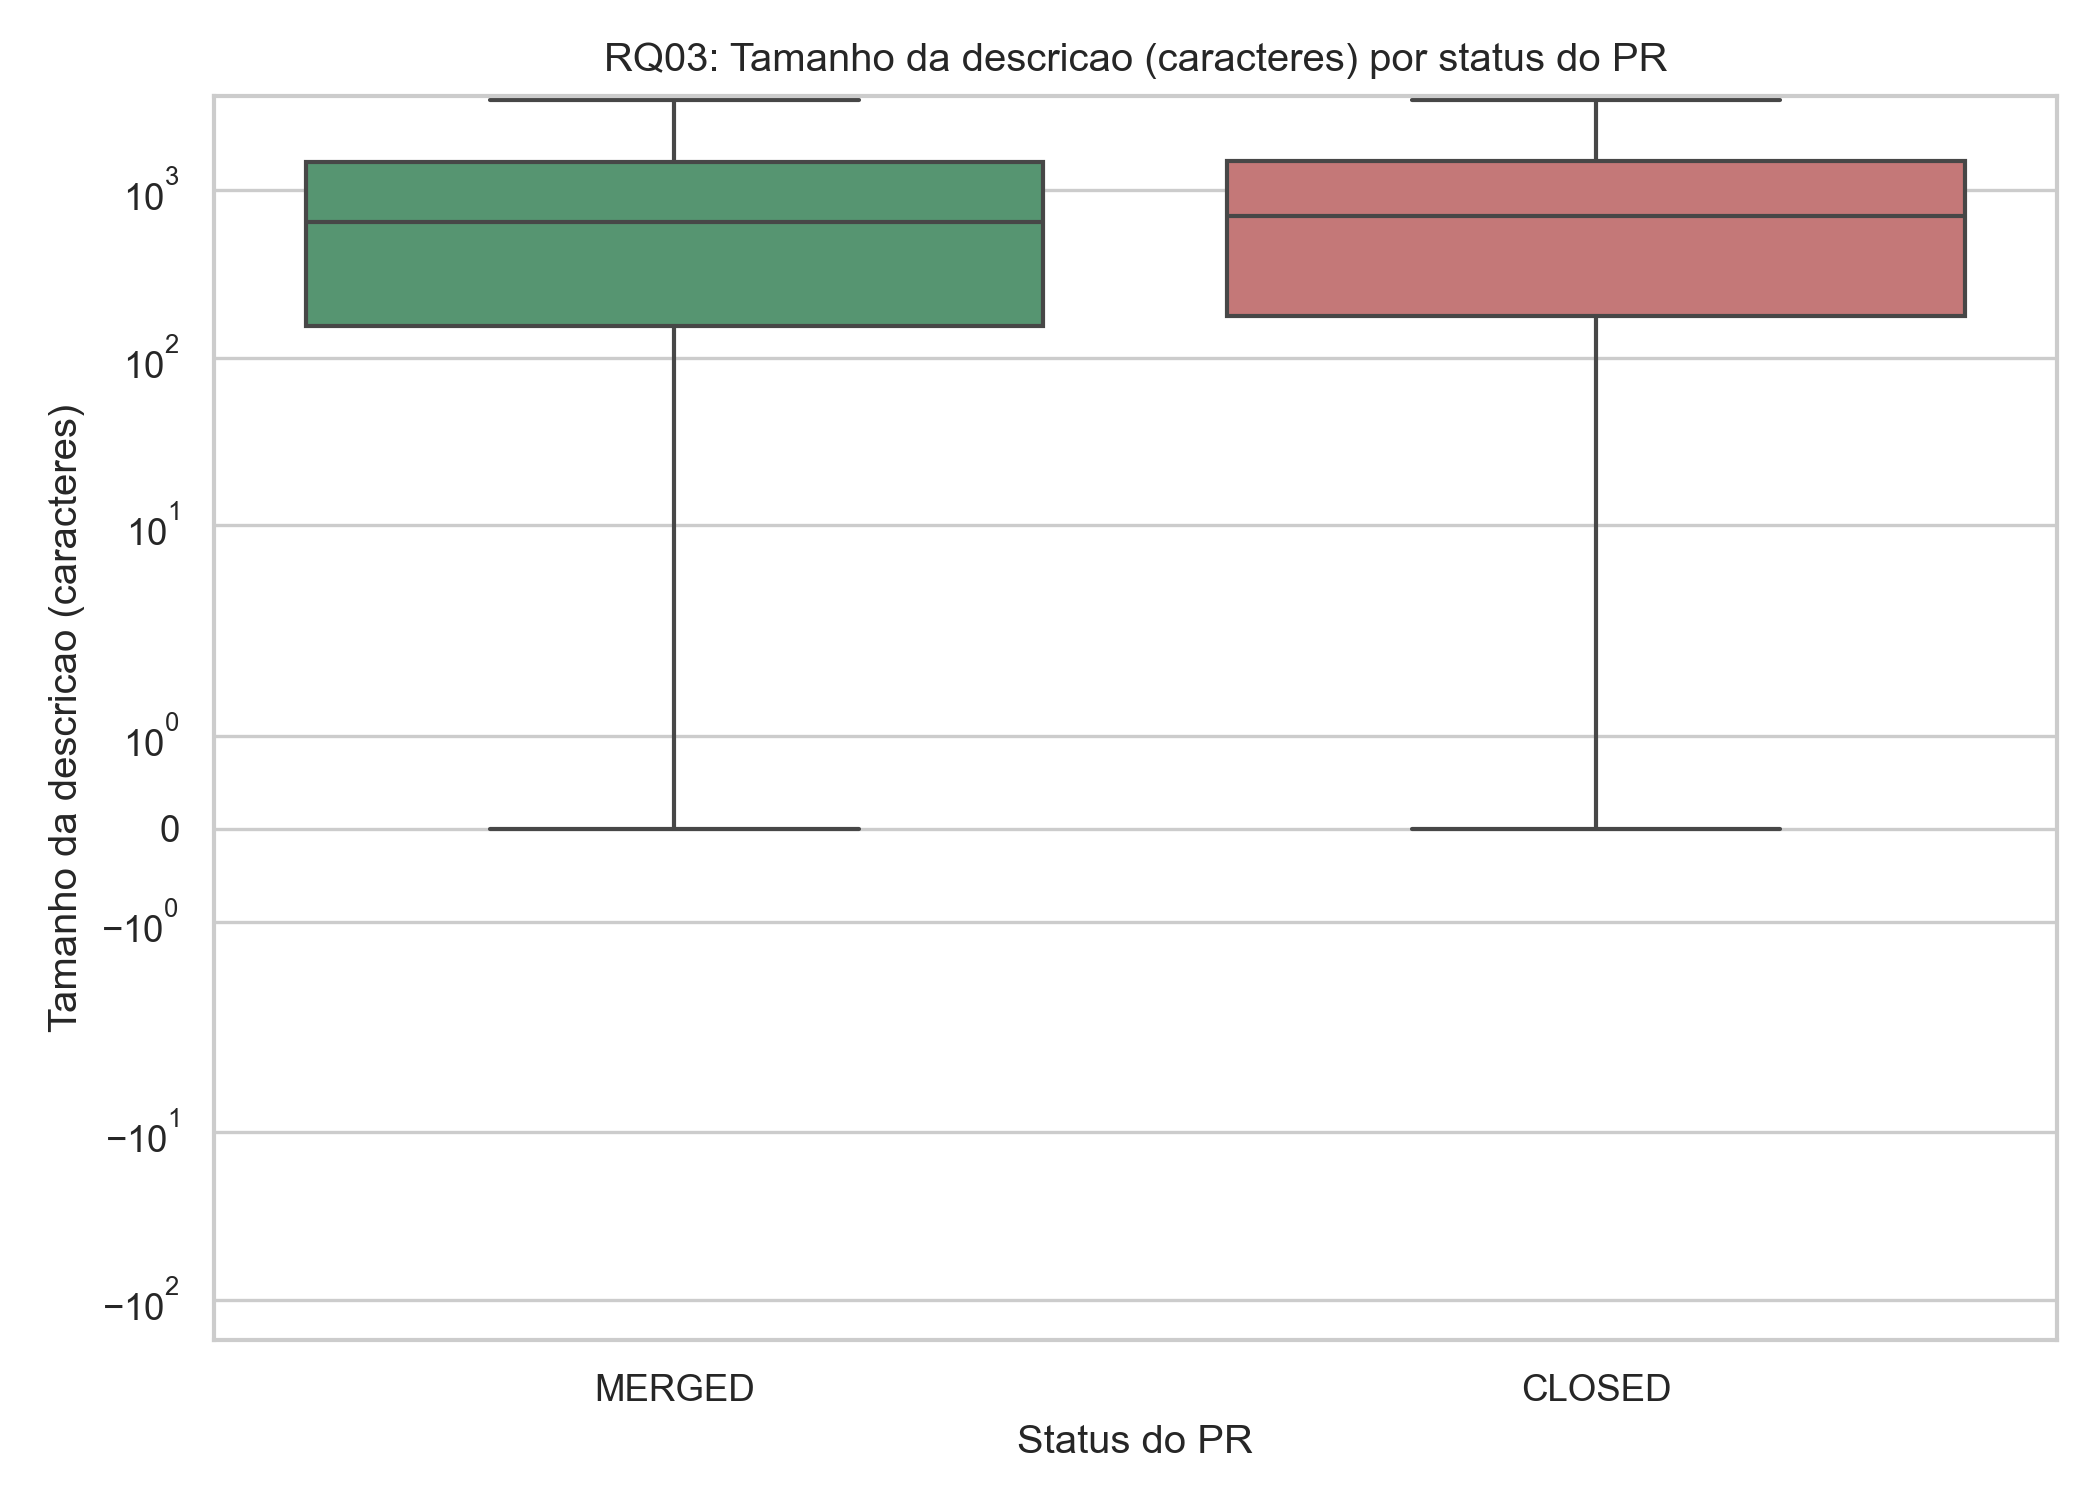
\includegraphics[width=0.78\textwidth]{../figures/rq03_boxplot_body_length_chars.png}
\caption{RQ03 - tamanho da descricao (caracteres)}
\label{fig:rq03_boxplot_body_length_chars}
\end{figure}

\subsection*{RQ04}
Para numero de participantes, a mediana entre PRs aceitos (MERGED) foi 2,00 e entre rejeitados (CLOSED) foi 2,00. A correla\c{c}\~ao de Spearman com o status (MERGED=1, CLOSED=0) resultou em $\rho = -0{,}0205$ ($p\,= 0{,}0194$). Veja a Figura~\ref{fig:rq04_boxplot_participants_count}. Para numero de comentarios, a mediana entre PRs aceitos (MERGED) foi 1,00 e entre rejeitados (CLOSED) foi 2,00. A correla\c{c}\~ao de Spearman com o status (MERGED=1, CLOSED=0) resultou em $\rho = -0{,}0808$ ($p\,< 0{,}0001$). Veja a Figura~\ref{fig:rq04_boxplot_comments_count}.

\begin{figure}[H]
\centering
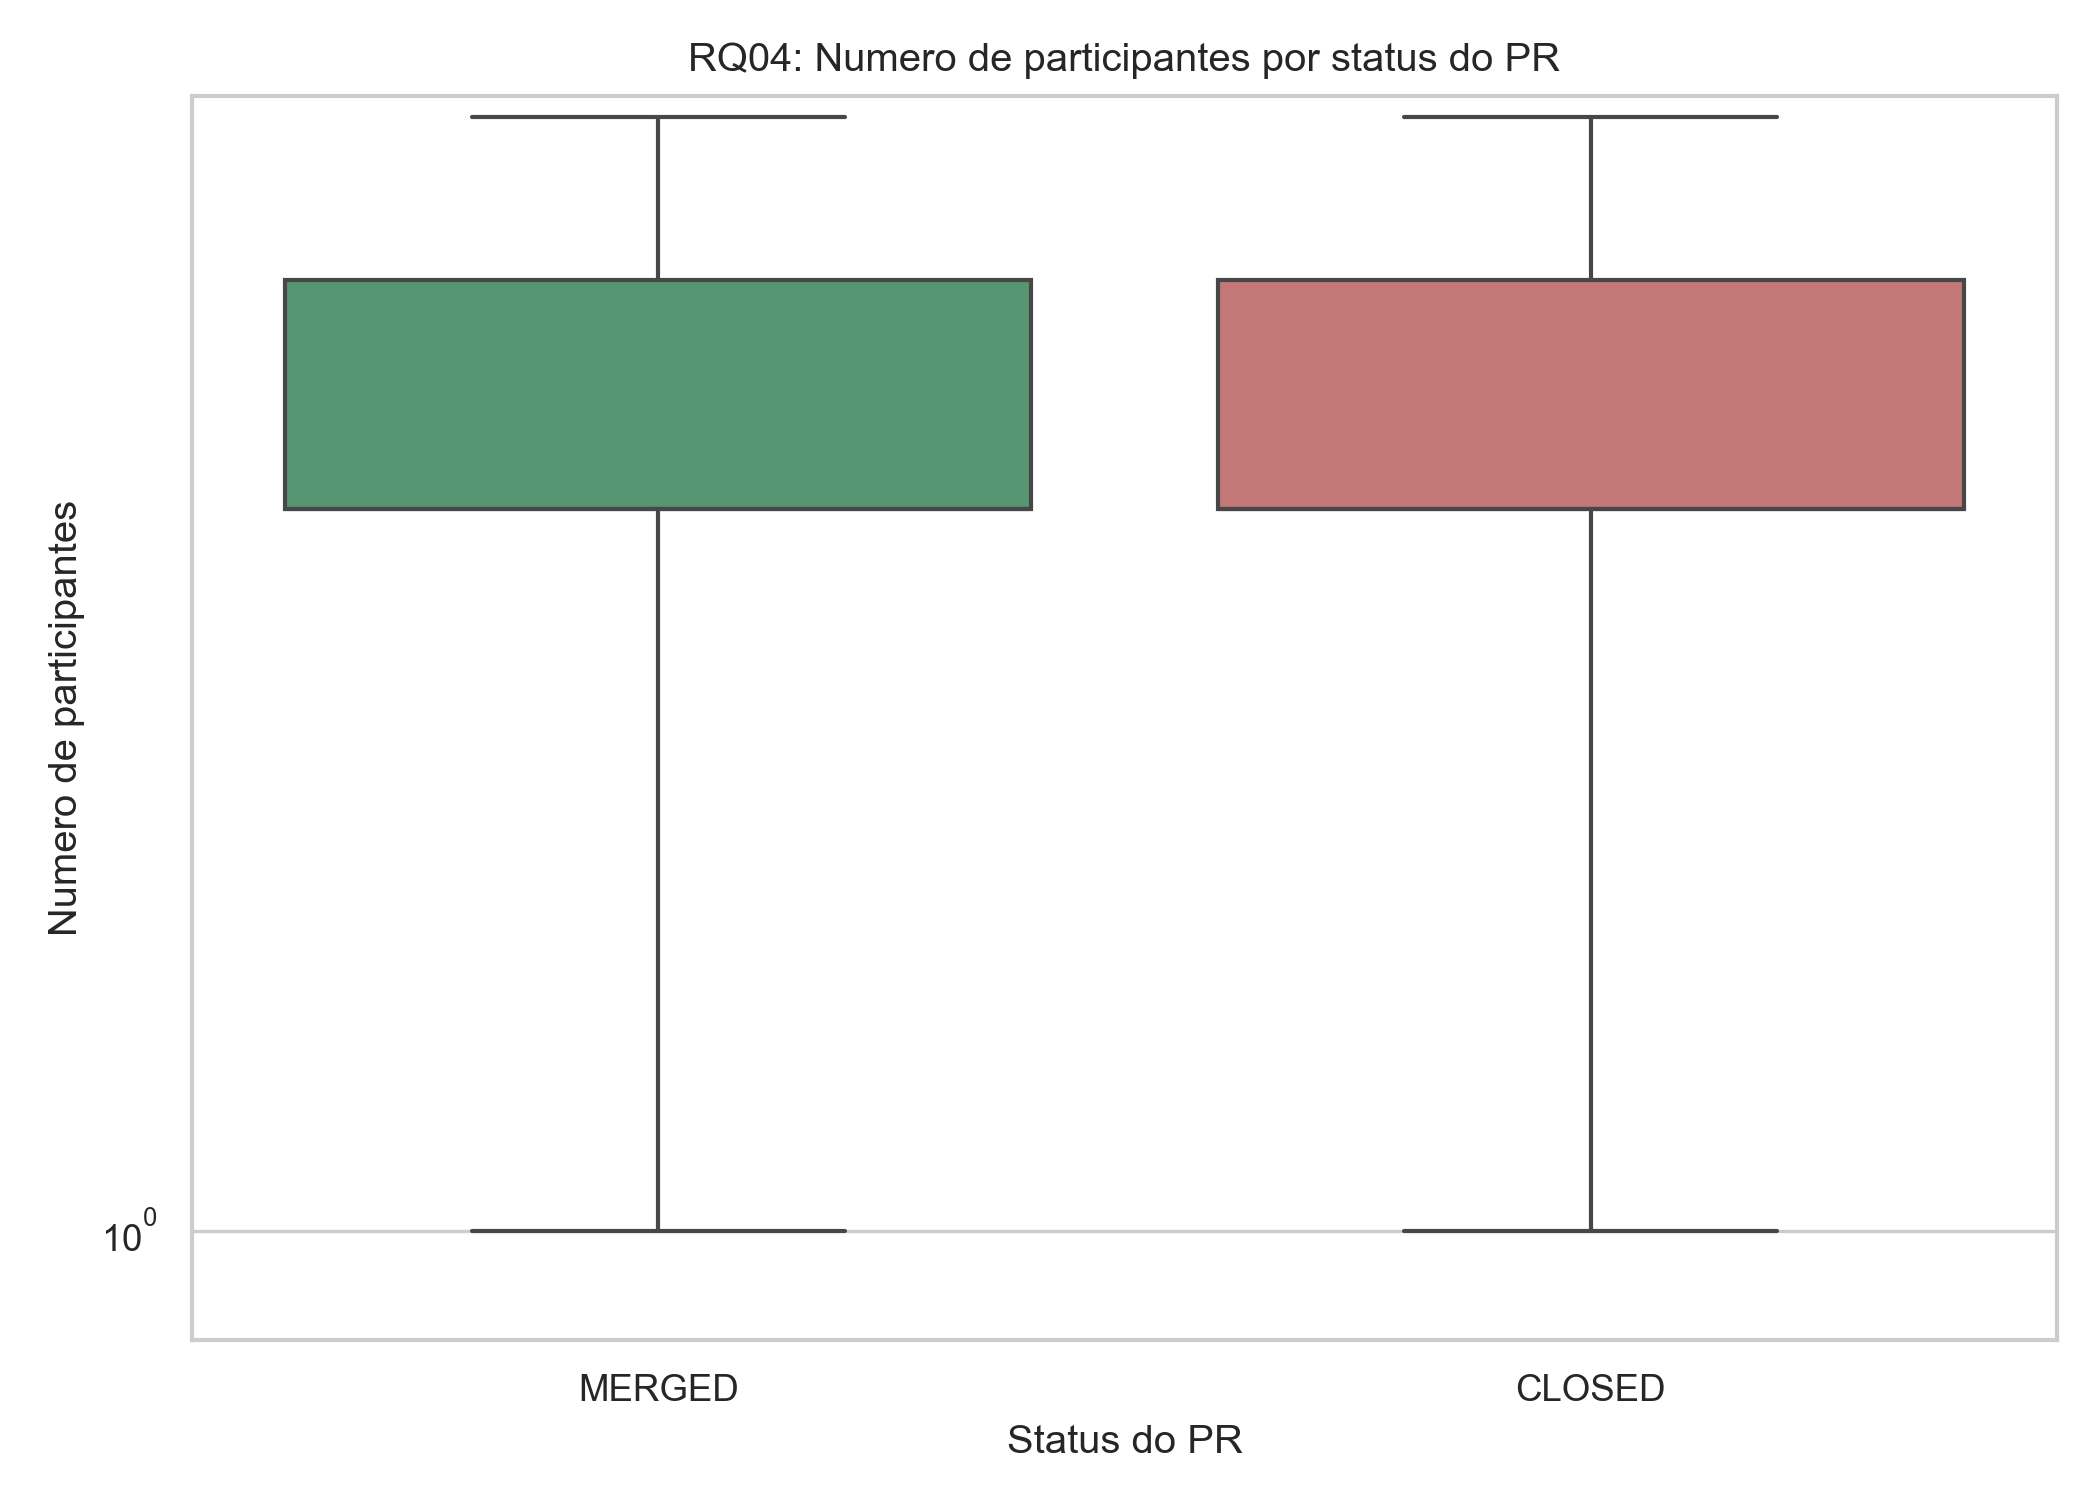
\includegraphics[width=0.78\textwidth]{../figures/rq04_boxplot_participants_count.png}
\caption{RQ04 - numero de participantes}
\label{fig:rq04_boxplot_participants_count}
\end{figure}

\begin{figure}[H]
\centering
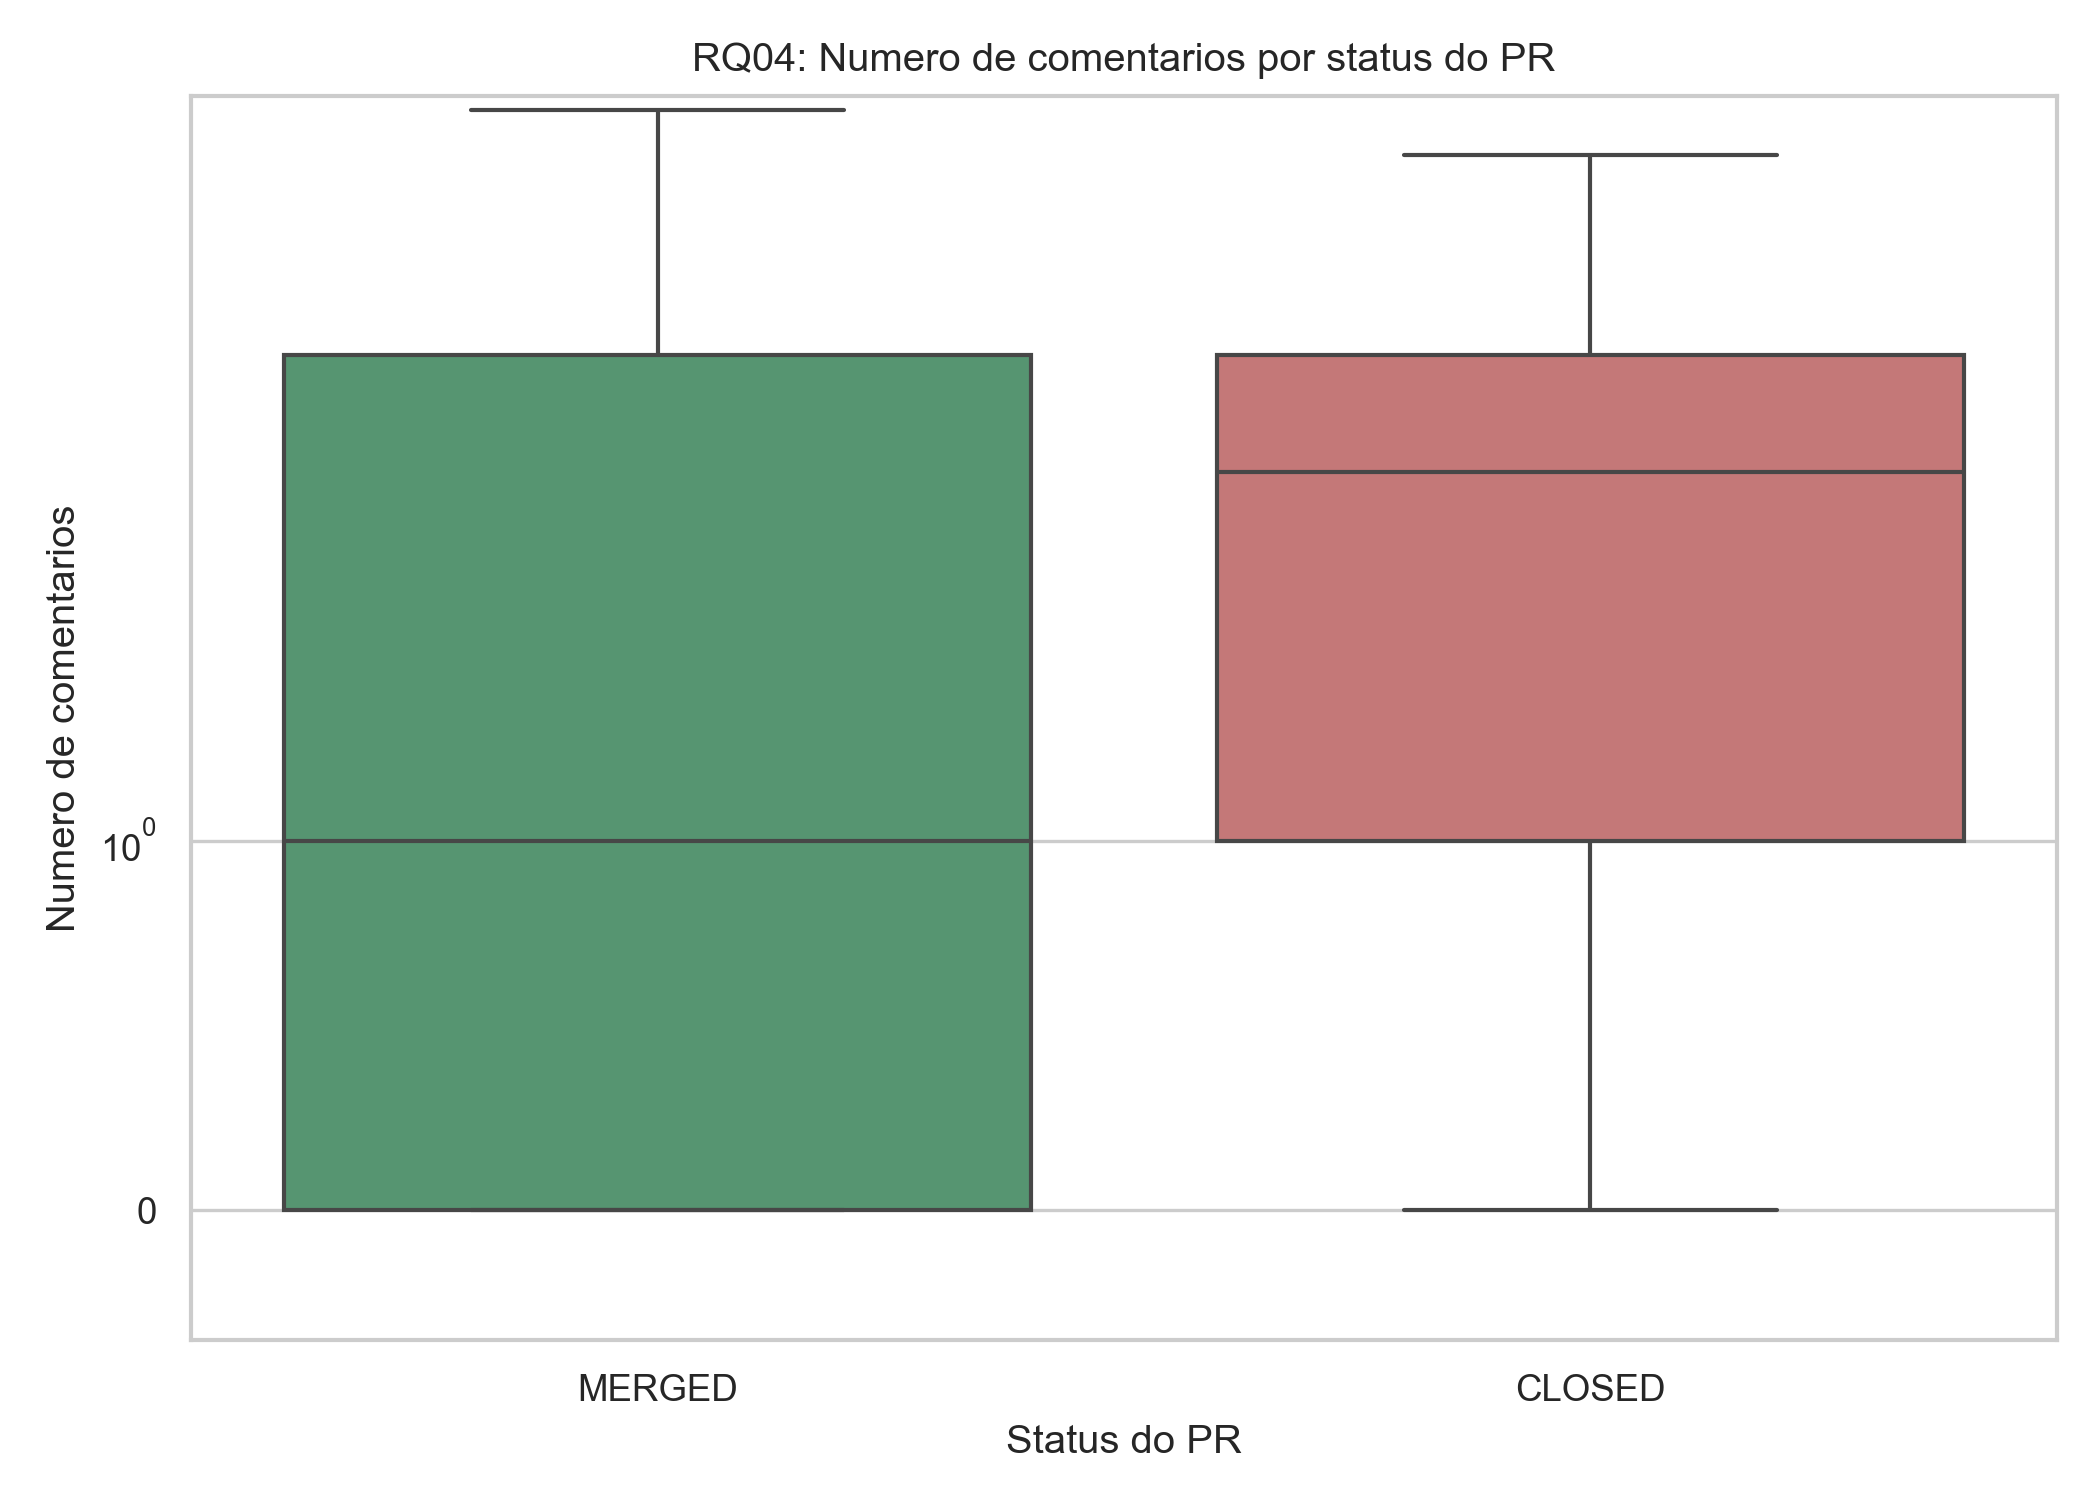
\includegraphics[width=0.78\textwidth]{../figures/rq04_boxplot_comments_count.png}
\caption{RQ04 - numero de comentarios}
\label{fig:rq04_boxplot_comments_count}
\end{figure}

\subsection{Dimens\~ao B -- N\'umero de revis\~oes}

\subsection*{RQ05}
Para arquivos alterados, a correla\c{c}\~ao de Spearman com o n\'umero de revis\~oes resultou em $\rho = 0{,}2450$ ($p\,< 0{,}0001$). Veja a Figura~\ref{fig:rq05_scatter_changed_files_vs_reviews}. Para linhas alteradas (additions + deletions), a correla\c{c}\~ao de Spearman com o n\'umero de revis\~oes resultou em $\rho = 0{,}2909$ ($p\,< 0{,}0001$). Veja a Figura~\ref{fig:rq05_scatter_lines_changed_vs_reviews}.

\begin{figure}[H]
\centering
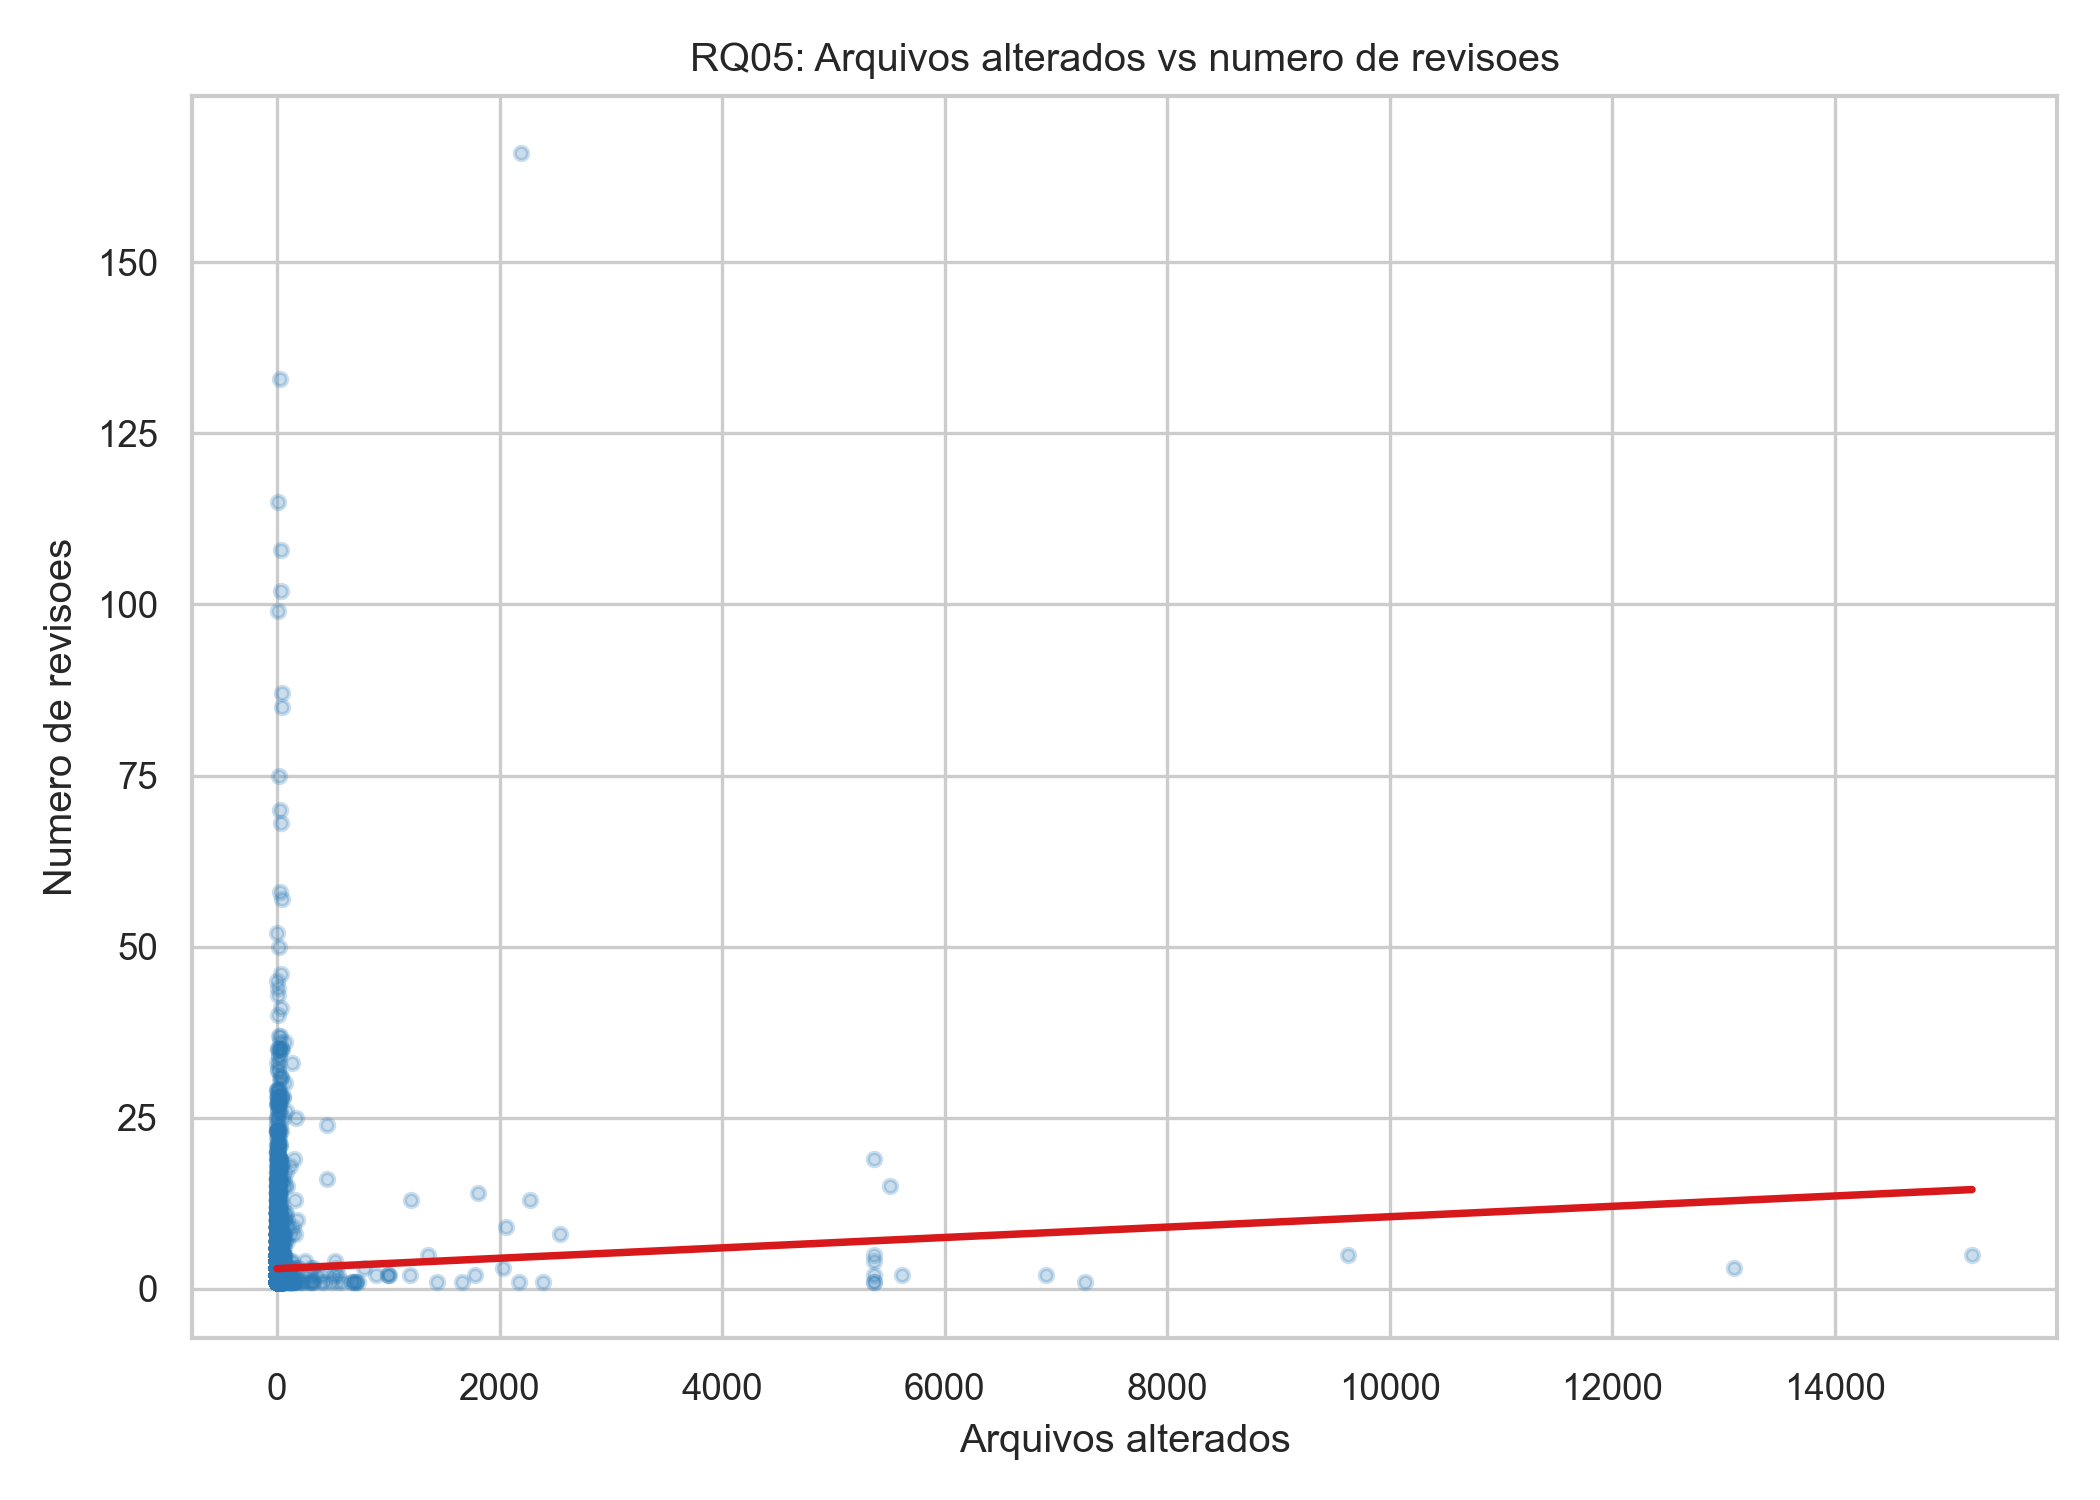
\includegraphics[width=0.78\textwidth]{../figures/rq05_scatter_changed_files_vs_reviews.png}
\caption{RQ05 - arquivos alterados}
\label{fig:rq05_scatter_changed_files_vs_reviews}
\end{figure}

\begin{figure}[H]
\centering
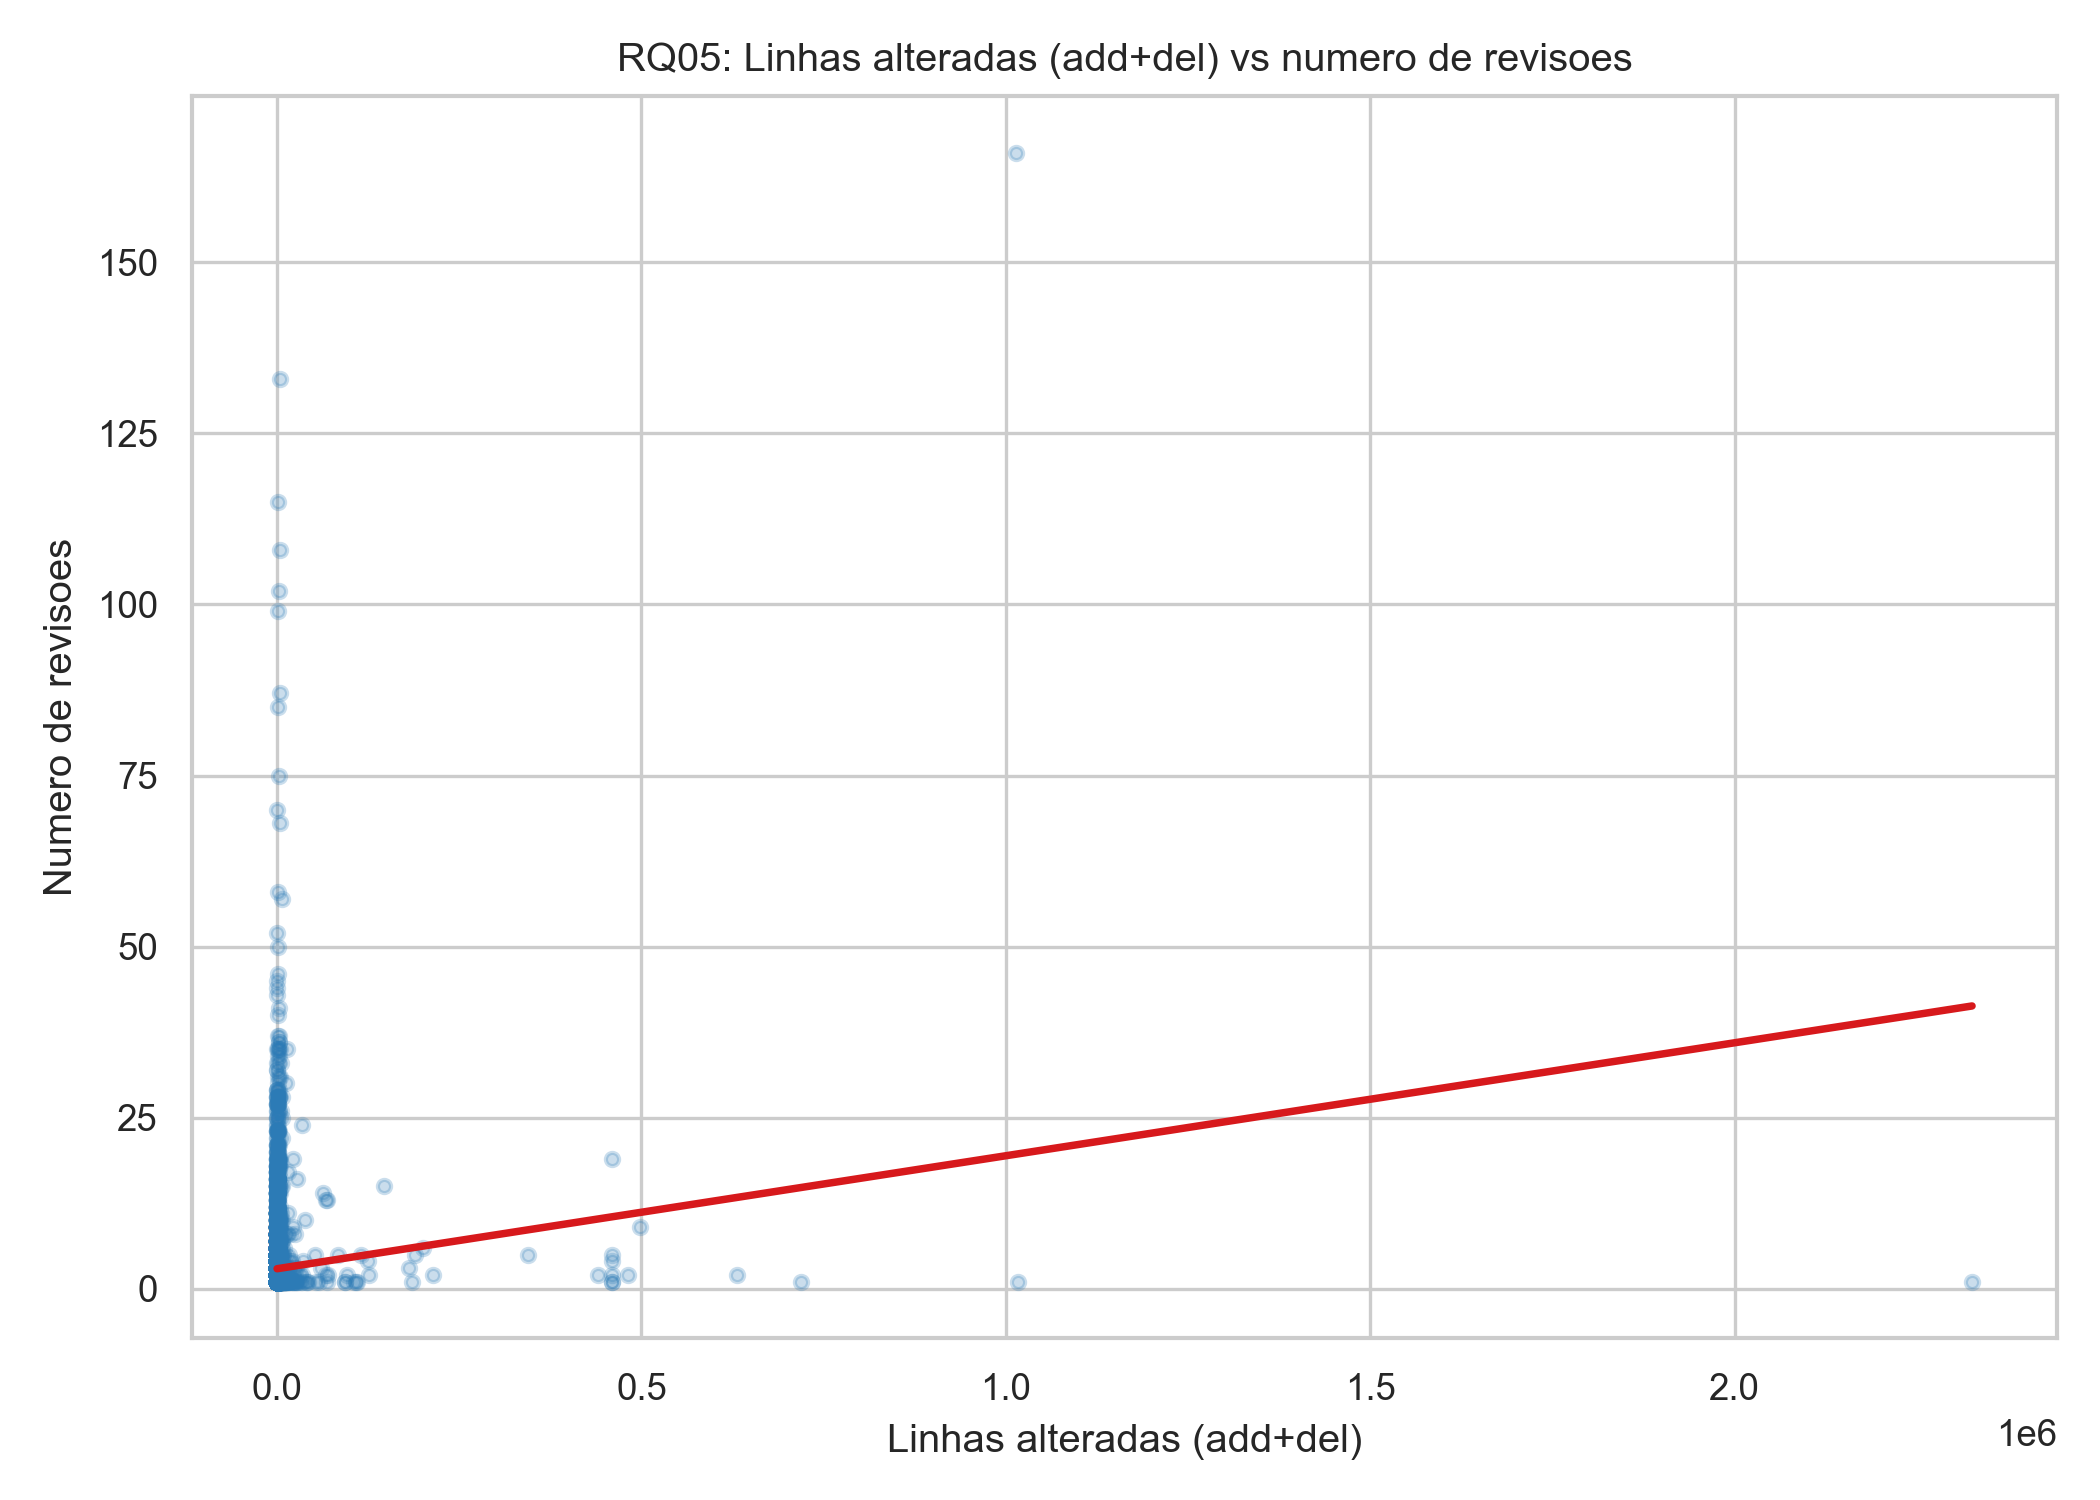
\includegraphics[width=0.78\textwidth]{../figures/rq05_scatter_lines_changed_vs_reviews.png}
\caption{RQ05 - linhas alteradas (additions + deletions)}
\label{fig:rq05_scatter_lines_changed_vs_reviews}
\end{figure}

\subsection*{RQ06}
Para tempo de analise (horas), a correla\c{c}\~ao de Spearman com o n\'umero de revis\~oes resultou em $\rho = 0{,}0777$ ($p\,< 0{,}0001$). Veja a Figura~\ref{fig:rq06_scatter_analysis_time_hours_vs_reviews}.

\begin{figure}[H]
\centering
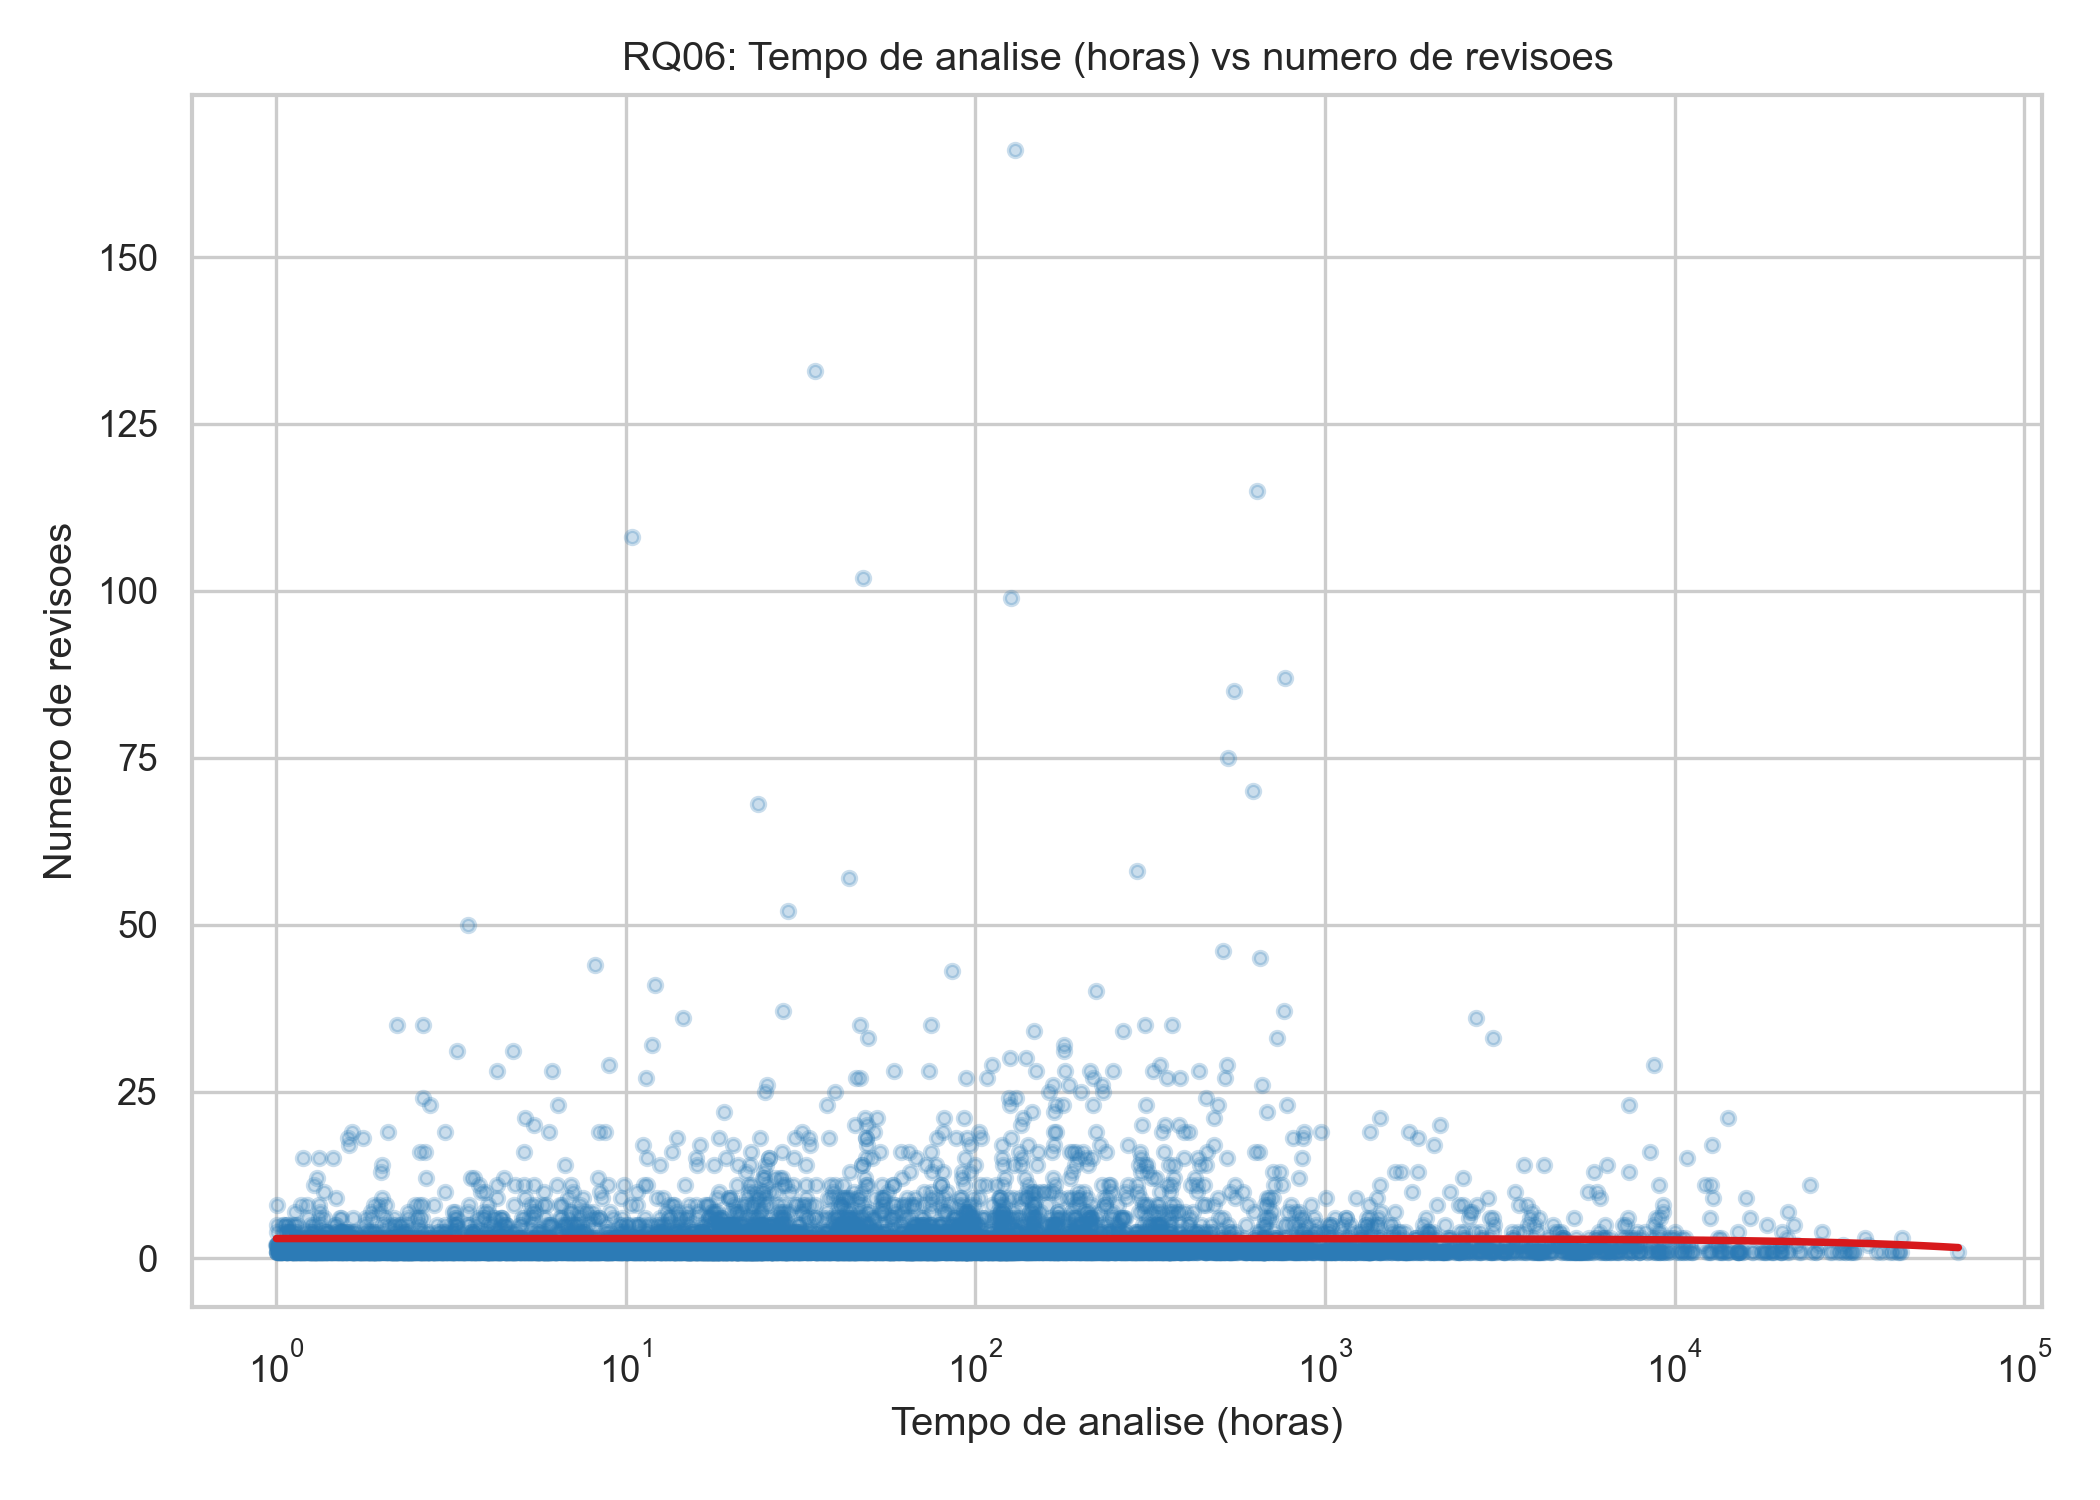
\includegraphics[width=0.78\textwidth]{../figures/rq06_scatter_analysis_time_hours_vs_reviews.png}
\caption{RQ06 - tempo de analise (horas)}
\label{fig:rq06_scatter_analysis_time_hours_vs_reviews}
\end{figure}

\subsection*{RQ07}
Para tamanho da descricao (caracteres), a correla\c{c}\~ao de Spearman com o n\'umero de revis\~oes resultou em $\rho = 0{,}1787$ ($p\,< 0{,}0001$). Veja a Figura~\ref{fig:rq07_scatter_body_length_chars_vs_reviews}.

\begin{figure}[H]
\centering
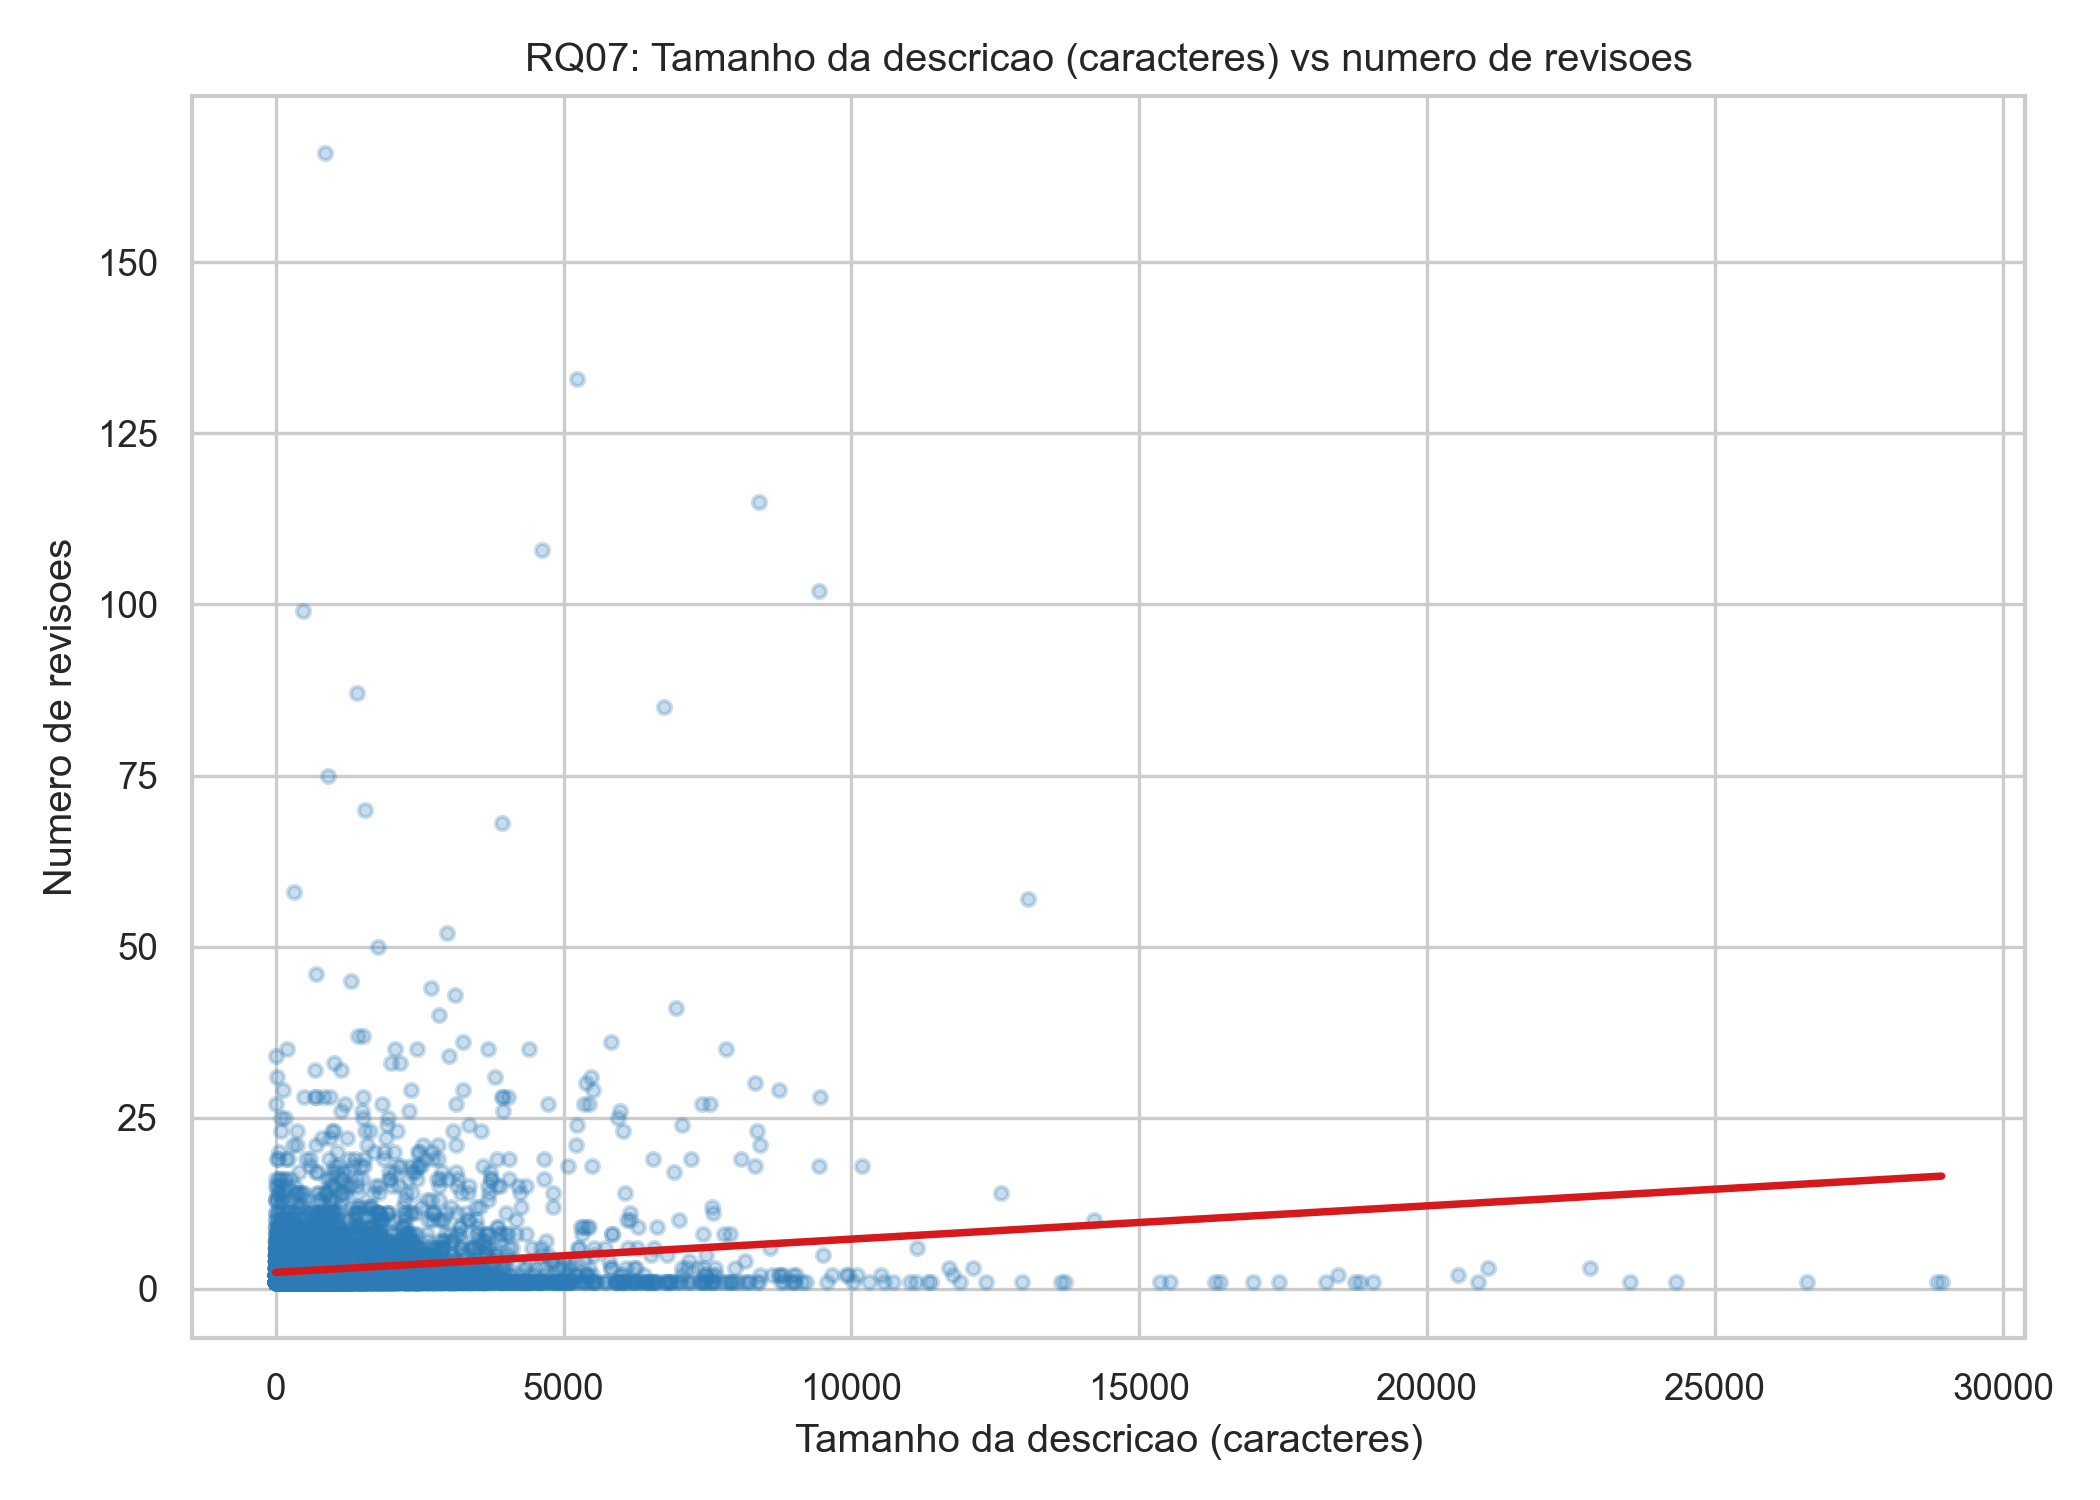
\includegraphics[width=0.78\textwidth]{../figures/rq07_scatter_body_length_chars_vs_reviews.png}
\caption{RQ07 - tamanho da descricao (caracteres)}
\label{fig:rq07_scatter_body_length_chars_vs_reviews}
\end{figure}

\subsection*{RQ08}
Para numero de participantes, a correla\c{c}\~ao de Spearman com o n\'umero de revis\~oes resultou em $\rho = 0{,}3504$ ($p\,< 0{,}0001$). Veja a Figura~\ref{fig:rq08_scatter_participants_count_vs_reviews}. Para numero de comentarios, a correla\c{c}\~ao de Spearman com o n\'umero de revis\~oes resultou em $\rho = 0{,}2899$ ($p\,< 0{,}0001$). Veja a Figura~\ref{fig:rq08_scatter_comments_count_vs_reviews}.

\begin{figure}[H]
\centering
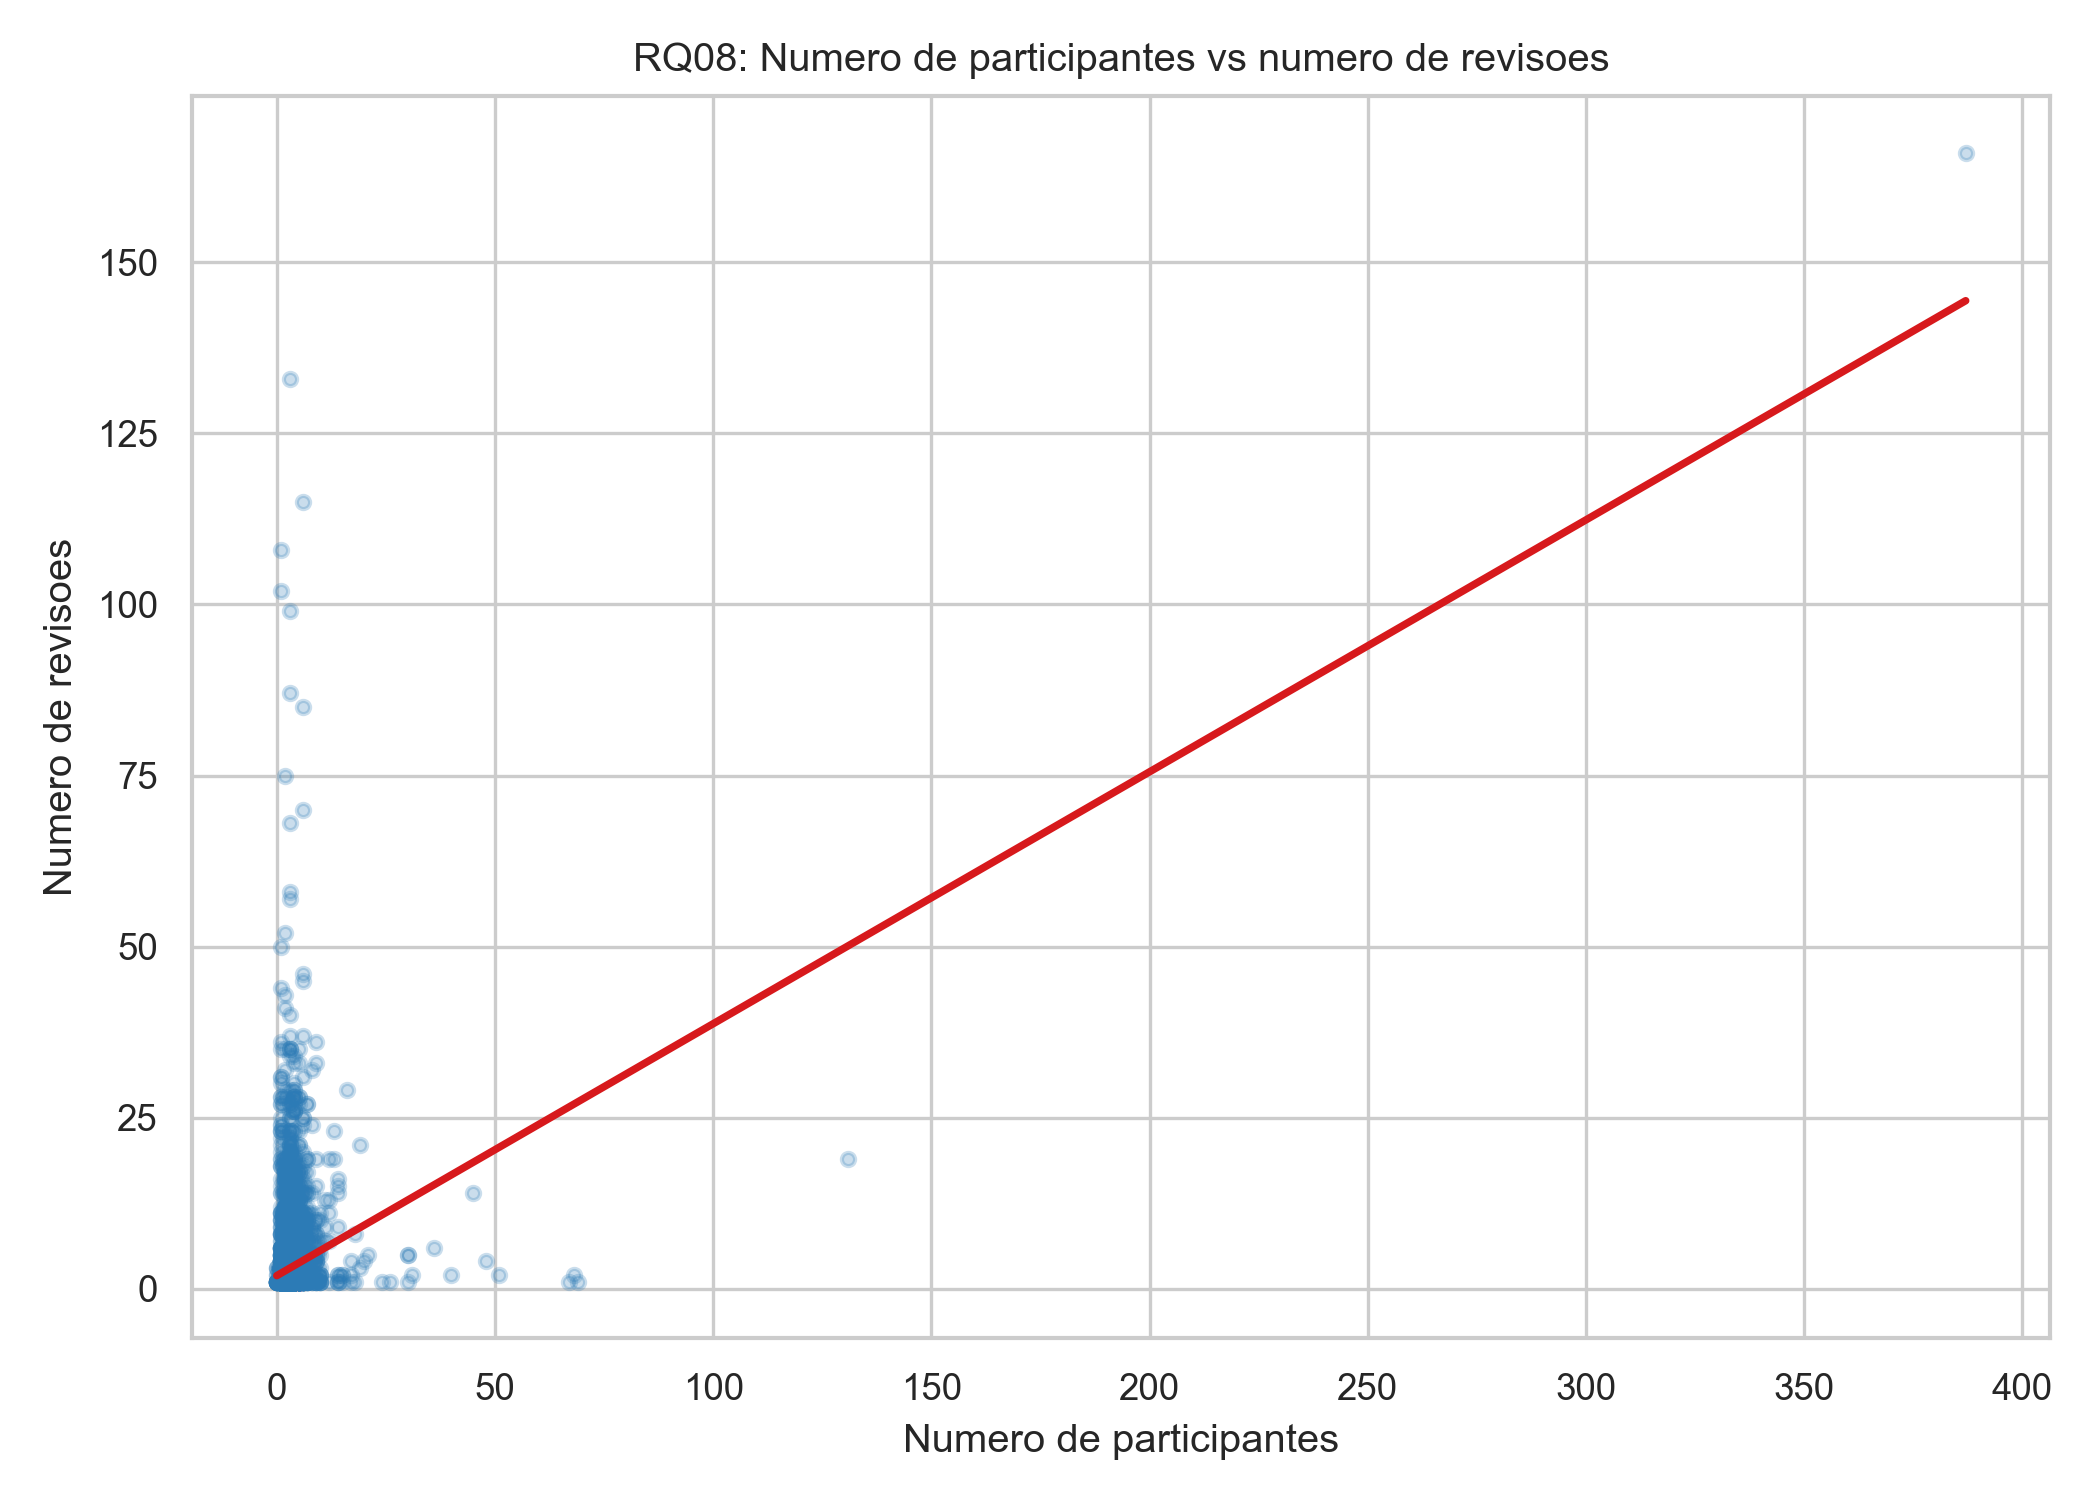
\includegraphics[width=0.78\textwidth]{../figures/rq08_scatter_participants_count_vs_reviews.png}
\caption{RQ08 - numero de participantes}
\label{fig:rq08_scatter_participants_count_vs_reviews}
\end{figure}

\begin{figure}[H]
\centering
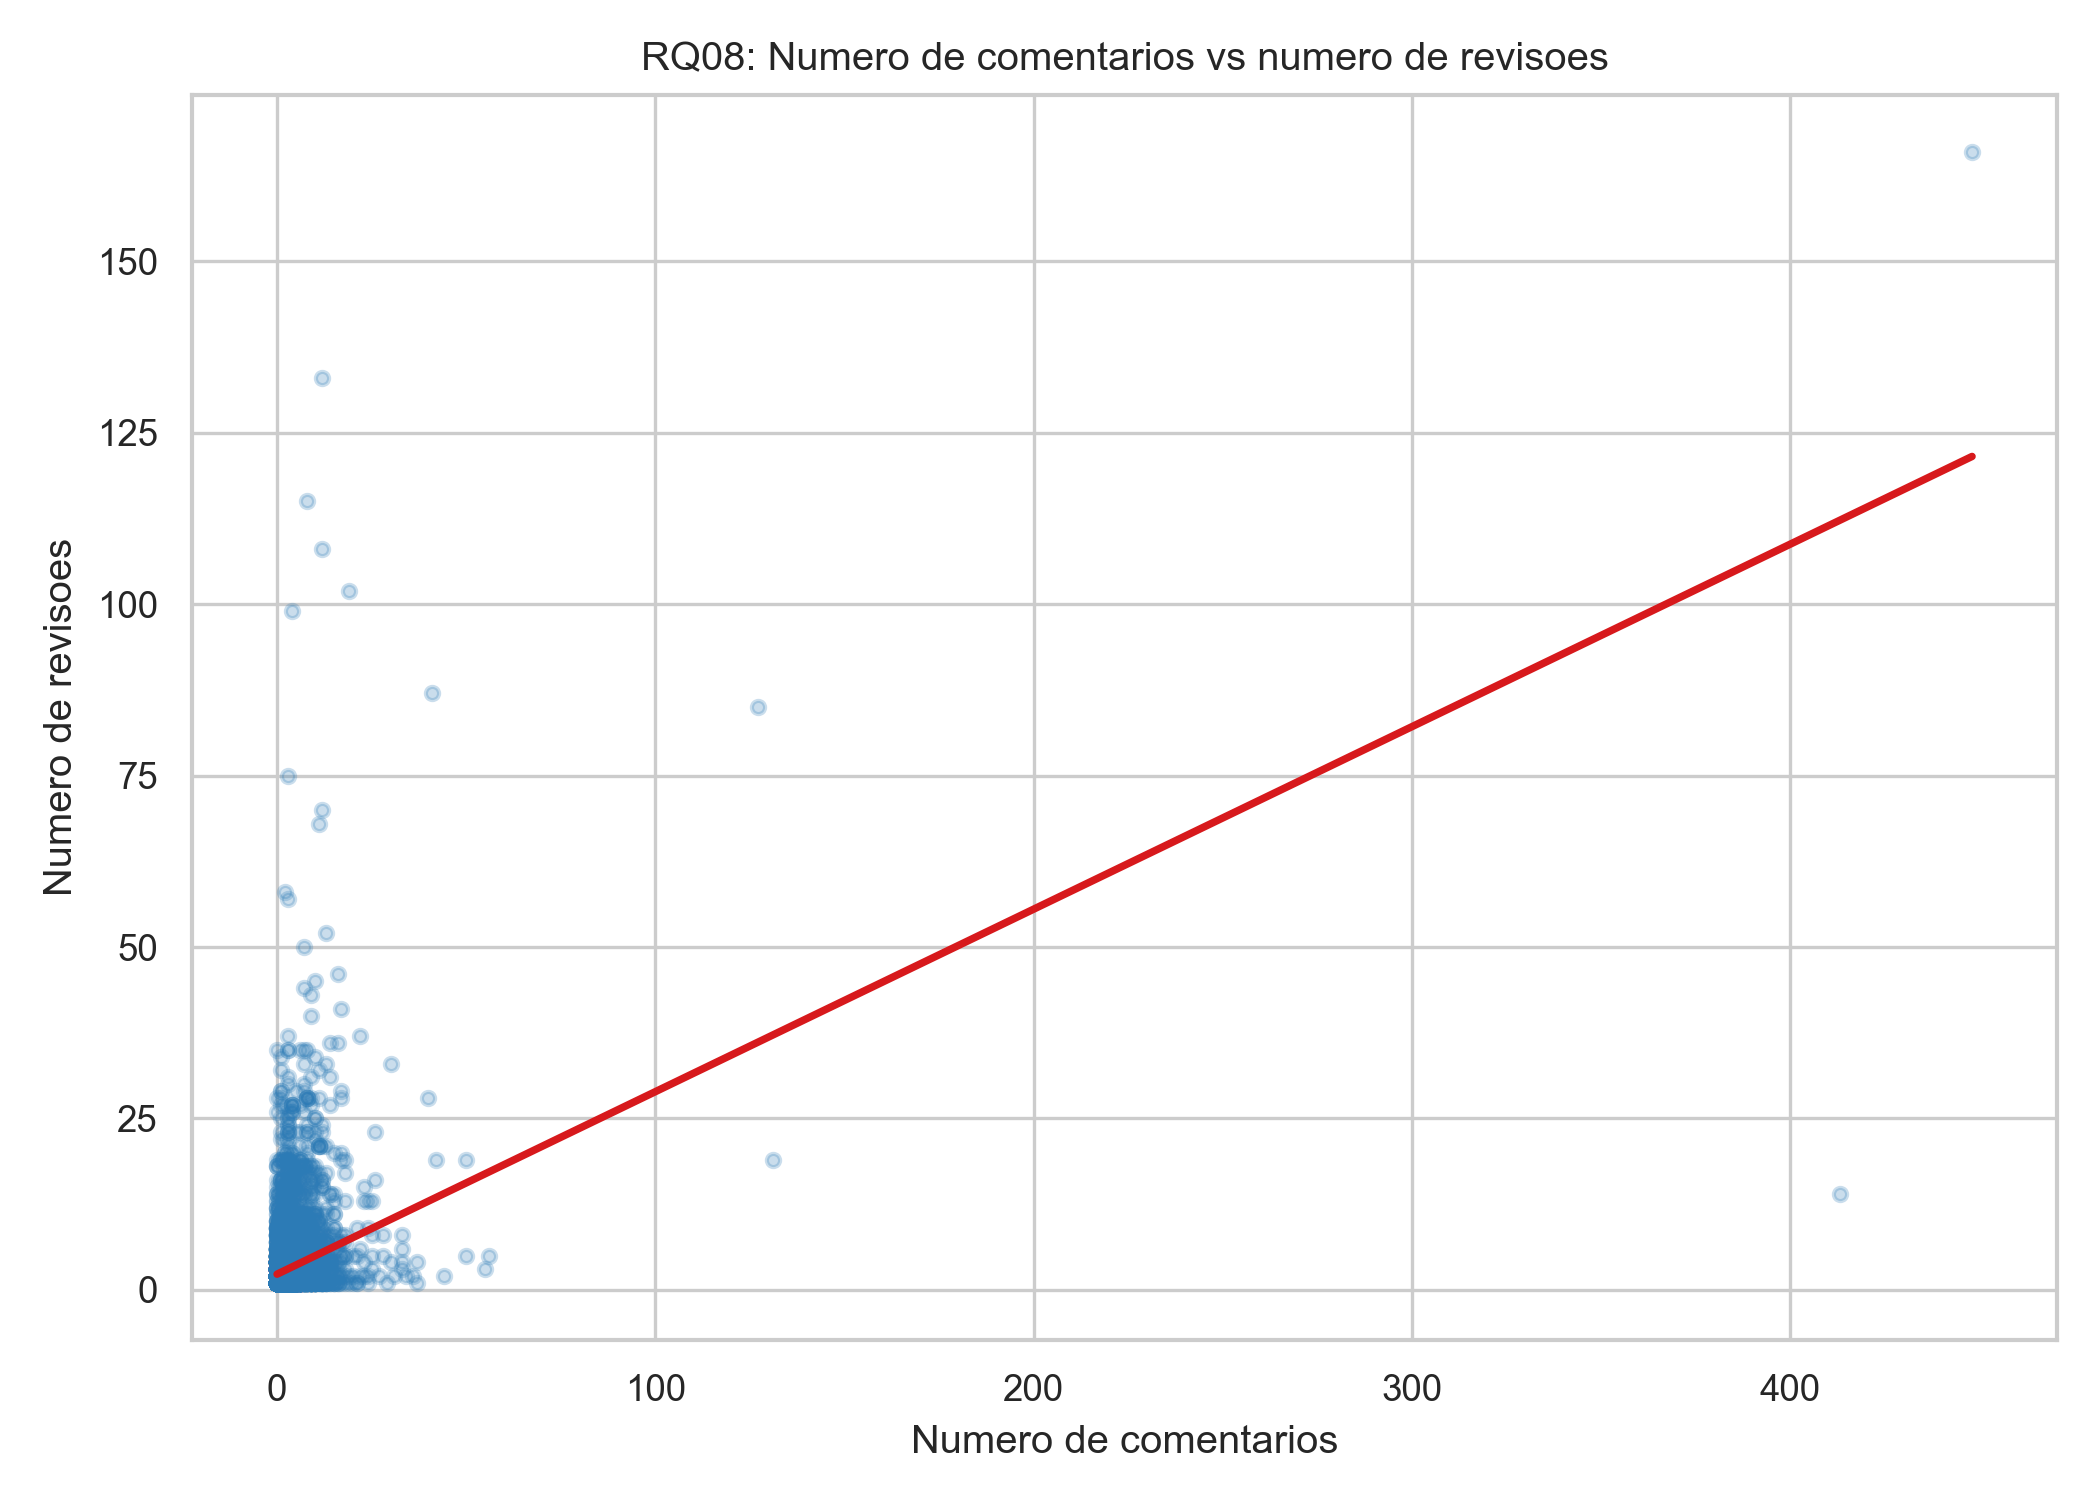
\includegraphics[width=0.78\textwidth]{../figures/rq08_scatter_comments_count_vs_reviews.png}
\caption{RQ08 - numero de comentarios}
\label{fig:rq08_scatter_comments_count_vs_reviews}
\end{figure}

\subsection{Vis\~ao geral das correla\c{c}\~oes}

\begin{figure}[H]
\centering
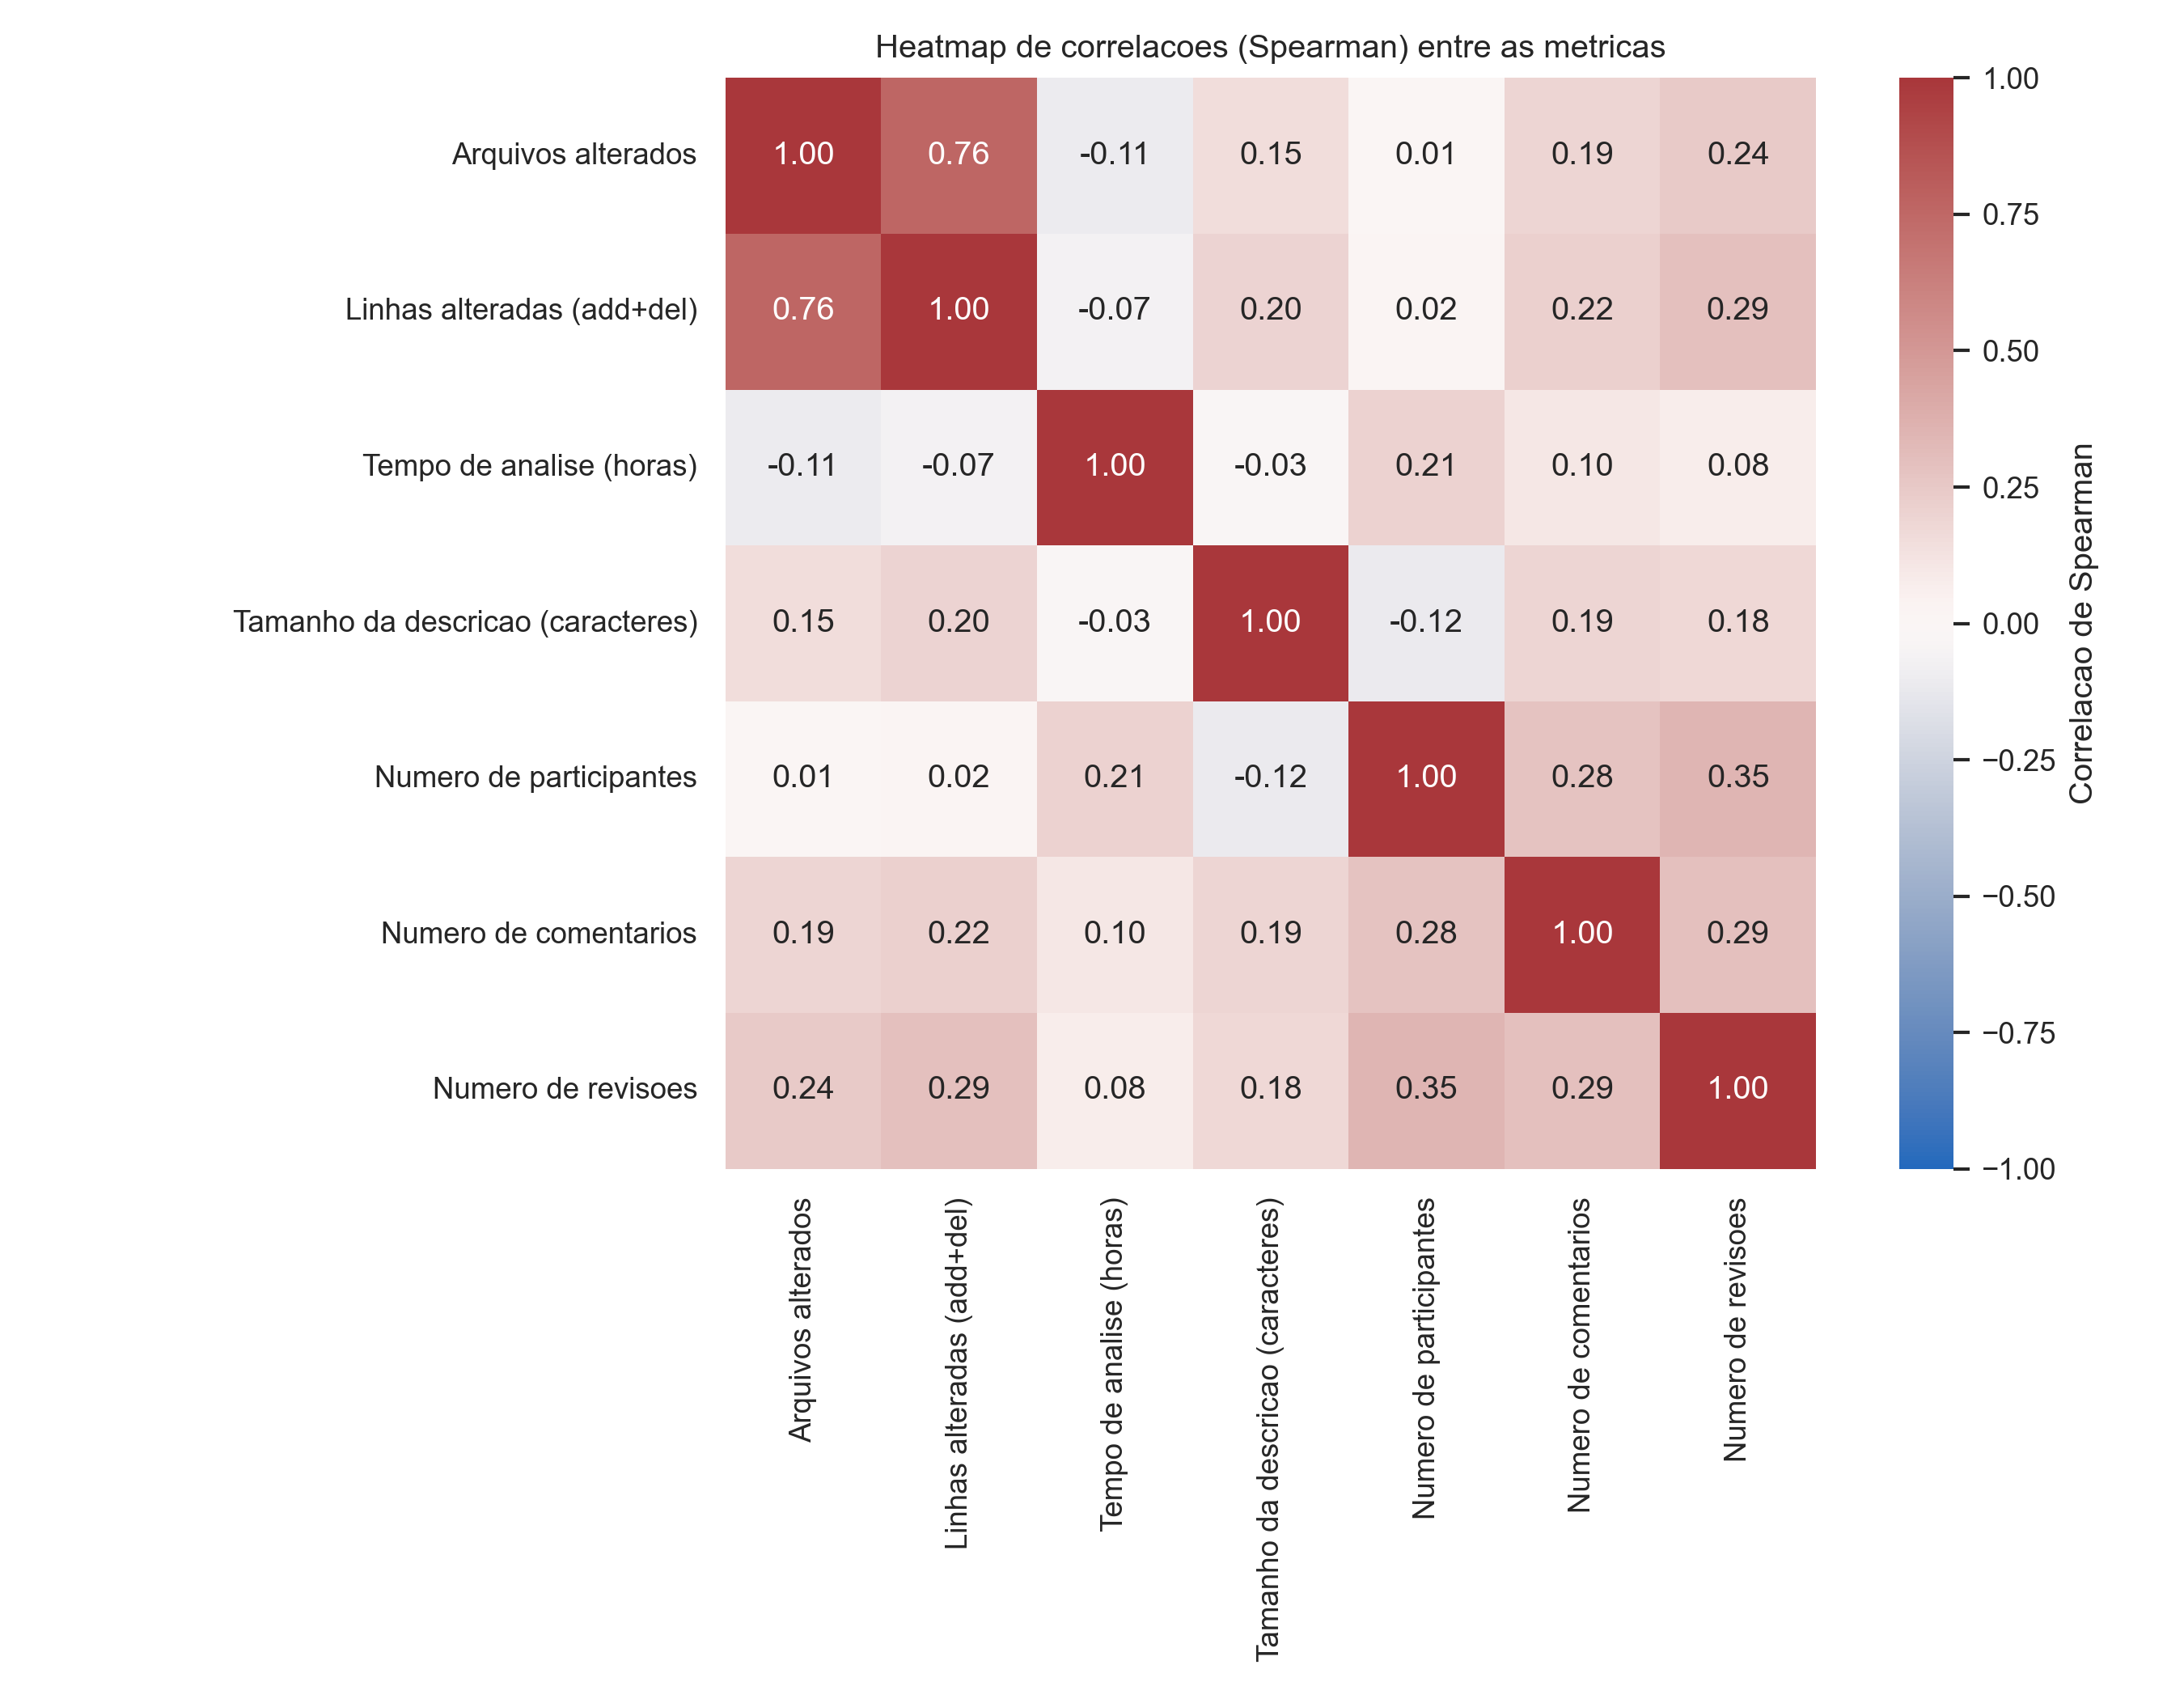
\includegraphics[width=0.85\textwidth]{../figures/heatmap_correlacoes.png}
\caption{Heatmap de correla\c{c}\~oes (Spearman) entre todas as m\'etricas.}
\label{fig:heatmap}
\end{figure}

\section{Discuss\~ao}

Nesta se\c{c}\~ao confrontamos as hip\'oteses iniciais com os valores observados.
Adotamos a seguinte conven\c{c}\~ao de intensidade para $|\rho|$: muito fraca ($< 0{,}1$),
fraca ($< 0{,}3$), moderada ($< 0{,}5$), forte ($< 0{,}7$) e muito forte ($\geq 0{,}7$).

\subsection*{RQ01}
Hipotese inicial: PRs maiores tendem a introduzir mais riscos e demandam revisao mais detalhada, logo esperamos que PRs com maior numero de arquivos alterados (e mais linhas modificadas) tenham menor probabilidade de serem aceitos. Para arquivos alterados, obtivemos rho = 0,1089 (intensidade fraca, direcao positiva); hipotese refutada. Para linhas alteradas (additions + deletions), obtivemos rho = 0,0299 (intensidade muito fraca, direcao positiva); hipotese nao se confirma (correlacao desprezivel).

\subsection*{RQ02}
Hipotese inicial: Esperamos correlacao negativa: PRs que permanecem muito tempo em revisao costumam indicar discussoes prolongadas ou problemas que tendem a culminar em fechamento sem merge. Para tempo de analise (horas), obtivemos rho = -0,2272 (intensidade fraca, direcao negativa); hipotese confirmada.

\subsection*{RQ03}
Hipotese inicial: Esperamos correlacao positiva: descricoes mais detalhadas fornecem contexto aos revisores e facilitam a aceitacao do PR. Para tamanho da descricao (caracteres), obtivemos rho = -0,0167 (intensidade muito fraca, direcao negativa); hipotese nao se confirma (correlacao desprezivel).

\subsection*{RQ04}
Hipotese inicial: Esperamos efeito misto: por um lado mais participantes e comentarios indicam atencao ao PR; por outro, podem refletir controversia e questionamentos, podendo correlacionar-se negativamente com o merge. Para numero de participantes, obtivemos rho = -0,0205 (intensidade muito fraca, direcao negativa); hipotese compativel (hipotese era mista). Para numero de comentarios, obtivemos rho = -0,0808 (intensidade muito fraca, direcao negativa); hipotese compativel (hipotese era mista).

\subsection*{RQ05}
Hipotese inicial: Esperamos correlacao positiva: PRs maiores tendem a passar por mais rodadas de revisao. Para arquivos alterados, obtivemos rho = 0,2450 (intensidade fraca, direcao positiva); hipotese confirmada. Para linhas alteradas (additions + deletions), obtivemos rho = 0,2909 (intensidade fraca, direcao positiva); hipotese confirmada.

\subsection*{RQ06}
Hipotese inicial: Esperamos correlacao positiva: quanto mais tempo em revisao, maior a oportunidade de novas revisoes ocorrerem. Para tempo de analise (horas), obtivemos rho = 0,0777 (intensidade muito fraca, direcao positiva); hipotese confirmada.

\subsection*{RQ07}
Hipotese inicial: Esperamos correlacao negativa (ou pequena): descricoes ricas reduziriam duvidas e, portanto, a necessidade de rodadas adicionais de revisao. Para tamanho da descricao (caracteres), obtivemos rho = 0,1787 (intensidade fraca, direcao positiva); hipotese refutada.

\subsection*{RQ08}
Hipotese inicial: Esperamos correlacao positiva: PRs com mais participantes e comentarios devem demandar mais revisoes. Para numero de participantes, obtivemos rho = 0,3504 (intensidade moderada, direcao positiva); hipotese confirmada. Para numero de comentarios, obtivemos rho = 0,2899 (intensidade fraca, direcao positiva); hipotese confirmada.

\section{Conclus\~ao}

Caracterizamos a atividade de \emph{code review} em 192 reposit\'orios populares do GitHub
analisando 12.979 \emph{Pull Requests} sob duas dimens\~oes: o \emph{feedback} final
(MERGED vs.\ CLOSED) e o n\'umero de revis\~oes. As principais observa\c{c}\~oes est\~ao
sumarizadas na Tabela~\ref{tab:rqs} e nas Figuras correspondentes a cada RQ.

Como limita\c{c}\~oes destacam-se: (i) o teto de 192 reposit\'orios e o limite
\texttt{PR\_LIMIT\_PER\_REPO} podem n\~ao representar comunidades de menor visibilidade;
(ii) o filtro de tempo $>$ 1h, embora elimine ru\'idos de \emph{bots}, pode descartar PRs
triviais leg\'itimos; (iii) o uso de \emph{Spearman} captura monotonicidade, mas n\~ao
implica causalidade. Trabalhos futuros podem incorporar an\'alises multivariadas e estratifica\c{c}\~ao
por linguagem ou dom\'inio do reposit\'orio.

\end{document}
